%% 
%% ACS project dissertation template. 
%% 
%% Currently designed for printing two-sided, but if you prefer to 
%% print single-sided just remove ",twoside,openright" from the 
%% \documentclass[] line below. 
%%
%%
%%   SMH, May 2010. 


\documentclass[a4paper,12pt ]{report}

%%
%% EDIT THE BELOW TO CUSTOMIZE
%%

\def\authorname{Nikola Mrk\v{s}i\'c\xspace}
\def\authorcollege{Trinity College\xspace}
\def\authoremail{nm480@cam.ac.uk}
\def\dissertationtitle{{Kernel Structure Discovery for ~~~ Gaussian Process Classification}}
\def\wordcount{8000}


%\usepackage{a4}
\usepackage{caption}
\usepackage{verbatim}
\usepackage{amsmath} 
\usepackage{amssymb,amsfonts}
\usepackage{hyperref}
\usepackage{mathtools}
\usepackage{amsthm}
\usepackage{booktabs}
\usepackage{multirow}
\usepackage{bm}
\usepackage{algpseudocode}
\usepackage{algorithm}
%\usepackage{adjustbox}
\usepackage{tocloft}
  %\usepackage[framed,numbered,autolinebreaks,useliterate]
\usepackage[margin=1.2in, bottom = 1.0in]{geometry}

  \usepackage{epsfig, epstopdf, graphicx,parskip,setspace,tabularx,xspace} 

\usepackage{preamble}
\usepackage{natbib}
\usepackage{color}
\usepackage{wasysym}
%\usepackage{subfigure}
\usepackage{bm}
  
  
\newtheorem{theorem}{Theorem}[section]
\newtheorem{proposition}[theorem]{Proposition}
\newtheorem{lemma}[theorem]{Lemma}
%\newtheorem{definition}[theorem]{Definition}
\newtheorem{examples}[theorem]{Examples}
\newtheorem{remarks}[theorem]{Remarks}
\newtheorem{corollary}[theorem]{Corollary}
\newtheorem{remark}[theorem]{Remark}
\newtheorem{example}[theorem]{Example}
\newtheorem{conjecture}[theorem]{Conjecture}
\newtheorem{question}[theorem]{Question}

\newcommand{\exedout}{%
  \rule{0.8\textwidth}{0.5\textwidth}%
}

%\newcommand{\cov}{\mathop{\mathrm{cov}}\nolimits}
\newcommand{\ex}{\mathbb{E}}
\newcommand*{\Scale}[2][4]{\scalebox{#1}{$#2$}}%
\newcommand{\f}{\mathbf{f}}

\renewcommand{\GP}{{GP}}

\hypersetup{
    colorlinks=false,
    pdfborder={0 0 0},
}

\captionsetup{skip=0pt}


%% START OF DOCUMENT
\begin{document}




%% FRONTMATTER (TITLE PAGE, DECLARATION, ABSTRACT, ETC) 
\pagestyle{empty}
\singlespacing
% title page information
\begin{titlepage} 

\begin{center}
\noindent
\huge
\dissertationtitle \\
\vspace*{\stretch{1}}
\end{center}

\begin{center}
\noindent
\huge
\authorname \\
\Large
\authorcollege      \\[24pt]

\includegraphics{CUni3.pdf}
\end{center}

\vspace{24pt} 

\begin{center}
\noindent
\large
{\it A dissertation submitted to the University of Cambridge \\ 
in partial 	fulfilment of the requirements for the Part III of \\ 
the Computer Science Tripos} 
\vspace*{\stretch{1}}
\end{center}

\begin{center}
\noindent
\Large \today
\end{center}



\begin{center}
\noindent
University of Cambridge \\
Computer Laboratory     \\
William Gates Building  \\
15 JJ Thomson Avenue    \\
Cambridge CB3 0FD       \\
{\sc United Kingdom}    \\
\end{center}





\end{titlepage} 

\newpage
\vspace*{\fill}

\onehalfspacing
\newpage
{\Huge \bf Declaration}

\vspace{24pt} 

I \authorname of \authorcollege, being a candidate for the Part III in
Computer Science, hereby declare that this report and the
work described in it are my own work, unaided except as may be
specified below, and that the report does not contain material that
has already been used to any substantial extent for a comparable
purpose.

\vspace{24pt}
Total word count: \wordcount

\vspace{60pt}
\textbf{Signed}: 

\vspace{12pt}
\textbf{Date}:


\vfill

This dissertation is copyright \copyright 2014 \authorname. 
\\
All trademarks used in this dissertation are hereby acknowledged.



\newpage
\vspace*{\fill}

\singlespacing
\newpage
{\Huge \bf Abstract}
\vspace{24pt}

This project was done at the Cambridge Machine Learning Group, as part of the larger effort to build an \emph{Automated Statistician}.

Given a data set, the Automated Statistician should run different methods to suggest interpretable hypotheses and the potential models to use for this data.

In this project, we have shown that automatic kernel discovery can be achieved for GP classification. We implemented a kernel structure search procedure inspired by previous work on regression by other members of the Group.

The evaluation on synthetic data sets demonstrated that the greedy procedure guided by approximate marginal likelihood can recover the underlying truth in these controlled experiments. The experiments on the four real-world biomedical data sets proved that our procedure achieves predictive performance on par with other recently proposed Bayesian models. Unlike the more complex models such as Additive GPs, our search procedure builds simple and interpretable kernels, similar to those that a human modeler might build when working on the given problem.

We have shown that the constructed kernels reveal interesting and interpretable patterns in the data. To represent these patterns, we developed functionality for visualising the posterior means of the composite kernels' components. These sets of plots correspond to the patterns identified in the data. This is the first step towards producing the automated reports for the end users, which we plan to pursue in further work.


\newpage


\vspace*{\fill}


\clearpage

\pagenumbering{roman}
\setcounter{page}{0}
\pagestyle{plain}
\tableofcontents

\clearpage

%\listoffigures
%\clearpage


%\listoftables
%\clearpage


\onehalfspacing

%% START OF MAIN TEXT 

\chapter{Introduction}
\pagenumbering{arabic} 
\setcounter{page}{1} 

\section{Building an Automated Statistician}


%This is the introduction where you should introduce your work.  In general the thing to aim for here is to describe a little bit of the
%context for your work --- why did you do it (motivation), what was the hoped-for outcome (aims) --- as well as trying to give a brief
%overview of what you actually did.

% It's often useful to bring forward some ``highlights'' into this chapter (e.g.\ some particularly compelling results, or a particularly interesting finding). 

%It's also traditional to give an outline of the rest of the document, although without care this can appear formulaic and tedious. Your call. 

\section{Contribution}

% Built a system for automatic kernel discovery for Gaussian Process classification...


\clearpage

%\chapter{Background} 

% A more extensive coverage of what's required to understand your work. In general you should assume the reader has a good undergraduate degree in computer science, but is not necessarily an expert in 
% the particular area you've been working on. Hence this chapter may need to summarize some ``text book'' material. 

% This is not something you'd normally require in an academic paper, and it may not be appropriate for your particular circumstances. Indeed, in some cases it's possible to cover all of the ``background'' 
%material either in the introduction or at appropriate places in the rest of the dissertation. 

\chapter{Background}

In this chapter, I will present the main ideas behind Bayesian inference, nonparametric Bayesian models and Gaussian Processes. I will present the main kernel families used for Gaussian Processes and outline the challenges encountered when performing classification using these models. 

\section{Bayesian Inference}

In classical probability theory, the probability of an event represents the relative frequency of its occurrence observed after $n$ repetitions of a well-defined random experiment. In such random experiments, an event has only two outcomes: it can either occur or not occur. The sample space $\omega$ represents all possible outcomes of the experiment, and an event is described as a subset of this space $\omega_e \subseteq \omega$. If $n_e$ is the number of event occurrences in $n$ trials, the probability of the event is defined as the limit of its relative frequency $\frac{n_e}{n}$ as $n$ tends to infinity. For example, when flipping a coin, the probability of a head outcome corresponds to the number of head outcomes divided by the total number of coin flips performed. % as $n \rightarrow \infty$. 

%\emph{The probability of an event is the ratio of the number of cases favourable to it, to the number of all cases possible when nothing leads us to expect that any one of these cases should occur more than any other, which renders them, for us, equally possible. }

This interpretation, known as the frequentist one, limits us to making observations and drawing conclusions only about those events we can repeat. Events such as `the world ends tomorrow' make no sense, as there can't be multiple samples of either positive or negative outcomes for this event: it happens only once. 

The Bayesian paradigm is more flexible, choosing to regard probabilities as \emph{subjective degrees of belief}. In Bayesian statistics, all types of uncertainty, including our own ignorance, are expressed using the formalism of probability theory \cite{gha12}.

When tackling a problem as a Bayesian, we first choose the likelihood model $ \Pr(D \mid \theta, M)$ which we believe can explain the data $D$ in the domain we want to model using some probabilistic model $M$. We also choose the prior distribution $\Pr(\theta)$ over the unknown parameters $ \theta $ of the likelihood model chosen. This model and its prior distribution subsume our subjective beliefs about the problem before we have observed any actual data, also known as the evidence. After observing some evidence, we modify our assumptions about the model parameters using Bayes' rule:

\begin{equation*} \Pr ( \theta \mid D, M) = \frac{ \Pr ( D \mid \theta, M) \Pr ( \theta \mid M) }{\Pr( D \mid M)} \end{equation*} 


Bayes' rule lies at the core of Bayesian inference. It provides a mathematically rigorous method for adapting our prior assumptions in light of new evidence, allowing us to move from our prior distribution $\Pr( \theta \mid M)$ to the updated posterior distribution $\Pr ( \theta \mid D, M) $. If more data becomes available, the posterior can be updated again: the current posterior becomes the prior and is updated using the new evidence $D'$ to arrive at the updated posterior distribution $\Pr ( \theta \mid D \cup D', M )$.

The likelihood function $\Pr(D \mid H, M)$ indicates how likely the data $D$ is to be observed assuming the probabilistic model $M$ with parameters $\theta$ for our data. Together with the prior $\Pr(\theta \mid M)$, the likelihood model describes the model used. The denominator $\Pr (D \mid M)$ is known as the \emph{marginal likelihood}. It is independent of the parameters $\theta$ so it does not affect the posterior distribution $\Pr (\theta \mid D, M)$. This means that the posterior is proportional to the likelihood times the prior. 

The intuition behind regarding the parameters as random variables lies in the Bayesian understanding of probability. Even though these values are not random, we model our uncertainty about their `true' values by assigning some probability mass to all of their potential values. Subsequently, when making predictions for some new instance $x$, we are in a position to consider all the available evidence by making decisions based on the weighted contributions of all realistic hypotheses $\theta$ to our prediction. The weights assigned to different hypotheses come directly from the posterior $\Pr(\theta \mid D, M)$ and are combined with the likelihood model $\Pr (x \mid \theta, M)$:

\begin{equation*}  \Pr(x \mid D, M) = \int_{\theta}{ \Pr(x \mid \theta, M) } \Pr ( \theta \mid D, M) d\theta  \end{equation*}

This is in direct opposition to the frequentist paradigm, which interprets the data as random samples drawn from some unknown underlying distribution. While a useful assumption to make, it is not actually true. Data is certain, and everything else in our inference procedure is uncertain: the prior, the likelihood model and the probabilistic model $M$ itself.  

The prior on the parameters is the result of our subjective judgement. This is not a weakness, but a strength of the Bayesian paradigm. All models have some assumptions built into them, allowing them to make predictions on the basis of the observed evidence. In the Bayesian paradigm, we are forced to make all of these assumptions explicit. Hence, if our model proves inadequate, it is not the fault of the inference mechanism, but of the flawed assumptions built into it \cite{gha12}. 

Another convenient property of Bayesian inference is that the effect of the prior decreases as more data becomes available, with the posterior mostly determined by the new evidence, assuming that the initial prior does not regard the observed evidence as entirely impossible. 

The value of marginal likelihood represents the probability of the evidence observed when the model parameters are integrated out, leaving just the dependency of the marginal likelihood on the probabilistic model $M$ used:

\begin{equation*} L ~=~ \Pr (D \mid M) = \int_{\theta}{\Pr(D \mid \theta, M) \Pr (\theta \mid M)} d\theta \end{equation*}

Very flexible models can not assign much probability to any data set observed, as they spread their probability mass to a wide array of possible observations. Conversely, overly rigid models are penalised for not being able to assign much probability mass to the evidence across the different parametrisations used. In both cases, this makes the marginal likelihood of these models lower than the marginal likelihood of models well suited to explaining the evidence. Hence, marginal likelihood can be used as the criterion for model ranking: the higher $L$ is, the better the model $M$ is at explaining the evidence $D$. 

The reason for this is that the marginal likelihood criterion subsumes an implicit Occam's razor for achieving a trade-off between the fit quality and model complexity \cite{zoubinoccam, rasmussen06}. Since model complexity determines the generalisation ability of the model, Bayesian models are less likely to overfit, that is include the noise in the data as part of the underlying signal, leading to poor performance on new observations. 

A fully Bayesian approach would introduce a prior over all possible models $M$ instead of picking one of them. However, choosing the set of all sensible models for a specific dataset is non trivial, and averaging their predictions may be difficult or even intractable. Bayesian nonparametric models are an efficient way to perform this averaging using families of very flexible probabilistic models. 
 %Bayesian methods do not fit parameters to the data in the same way that frequentist models do, so there can be no overfitting in the same sense.

% Is this what the Bayesian does, or should one also intergrate out the model?
% Likelihood as noise model??

\section{Bayesian nonparametric models}

In statistics, parametric models represent collections of probability distributions which can be described using a finite number of parameters. Given the observed evidence $E$, one chooses (trains) the model parameters $\mathbf{\theta}$, which then contain information extracted from $E$ to be used for subsequent inference. In other words, having trained the parameters, subsequent predictions are independent of the evidence observed \cite{gha12}: 
\begin{equation*}	\Pr ( x \mid \mathbf{\theta}, E ) = 	\Pr ( x \mid \mathbf{\theta} )	\end{equation*}
For modelling complicated datasets with complex relationships between its features, one has to use increasingly sophisticated models. In general, the larger the number of parameters is, the more flexible the model built becomes. 

Nonparametric models reject the notion of using a finite set of parameters to describe the distribution of the data: the larger the data sample is, the more parameters we need to describe it. This idea contradicts the standard Bayesian formulation, where the prior and posterior distributions are defined over a fixed parameter space. 

Using a fixed number of parameters limits the complexity of our model and prevents us from capturing all the structure available in large and complicated data sets. Bayesian nonparametric (BNP) models overcome this limitation by transitioning to an infinite-dimensional parameter space, capable of dealing with data sets of arbitrary sizes. In general, the number of parameters utilised grows with the size of the data set available. This means that BNP models are defined over an infinite parameter space but can be evaluated using a finite subset of these to explain any given data sample \cite{orbanzteh}. Inference is performed by marginalising out the surplus dimensions over the prior, leaving only those dimensions which carry information relevant to explaining the data. 

The \emph{nonparametric} attribute in BNP models is somewhat misleading, as not only are these models not without parameters, but they have an infinite number of them. The infinite set of parameters is usually represented using a function or a probability measure \cite{orbanzteh}, where the function . Defining a prior over these requires the use of distributions on functions, measures and other infinite-dimensional objects. These distributions are known as stochastic processes, and many of the resulting BNP models, such as the Dirichlet, Beta and Gaussian processes bear the name of the underlying stochastic process. One can arrive at many of the standard BNP models, including the Gaussian process, by letting the number of parameters tend to infinity in standard parametric models such as the multivariate normal distribution. 

Computing the posteriors of the stochastic processes embedded in BNP models is non trivial, due to their infinite number of parameters. However, most BNP models have analytically tractable posteriors. This means that the unused parameters can be integrated out efficiently, leaving us with a finite number of parameters to handle using standard techniques such as Markov chain Monte Carlo, variational inference or message passing algorithms \cite{orbanzteh}. The techniques chosen to handle inference using these models generally follow the same trade-offs between speed and accuracy as their parametric counterparts. 

The theoretical properties of BNP models are harder to express and reason with. Proving convergence and consistency is more difficult, and properties such as the \emph{exchangeability} of the observations must be established. While the theory behind BNP models is more sophisticated and demanding than for the analogous parametric cases, the resulting models are far more flexible and provide an alternative to model selection from a parametrised family of models. Many of the machine learning techniques widely used today are non-parametric: kernel methods, SVMs, Gaussian processes, etc. %Deep neural networks also come close to being non-parametric, having a huge number of units, usually exceeding the number of parameters in BNP models such as Gaussian processes. 

\section{Gaussian Processes} 

\textbf{Definition} A collection of random variables $\{ X_t, t \in T \}$ is a Gaussian process if any finite dimensional subset of these random variables has a consistent joint Gaussian distribution \cite{rasmussenGPs}.

The simplest way of thinking about the Gaussian process is as of an infinite-dimensional generalisation of the multivariate Gaussian distribution. The Gaussian distribution is fully specified by its mean vector $\mu$ and covariance matrix $\Sigma$. For the sake of building intuition, one may regard any function $\mathbf{f}$ as an infinitely long vector, indexed by the elements of the index set $T$. Then, for any choice of distinct values $\{t_1 \ldots t_k\} \subset T$, the \emph{random vector} $ \mathbf{f} = (f_{t_1}, \ldots, f_{t_k})^\top $ has a multivariate distribution with mean $\ex(\mathbf{f}) = \mu $ and covariance matrix $\cov(\mathbf{f}, \mathbf{f}) = \Sigma$, that is: 

\begin{equation*} \mathbf{f} ~ = ~ (f_{t_1}, \ldots, f_{t_k} )^\top ~ \sim ~ \mathcal{N}(\mu, \Sigma) \end{equation*}

Letting the length of this vector tend to infinity, we arrive at the Gaussian process: the finite random vector $\mathbf{f}$ becomes a function and the mean vector and the covariance matrix become functions $m(x)$ and $K(x_1, x_2)$. We will denote draws from the resulting stochastic process as:

\begin{equation*} \mathbf{f} ~ \sim ~ \GP(m, K) \end{equation*}

where the values ${f(t_1), \ldots, f(t_k)}$ are now joint Gaussian random variables for any finite subset of $T$. A common assumption is that these random variables have mean zero, which simplifies calculations without loss of generality. This assumption allows the properties of the Gaussian process to be fully specified by the covariance function $K$. In practice, this can be implemented by centring the examples in the data set during the pre-processing stages. 

Given $\GP(m, K)$ and a finite set of $N$ observations $ \mathbf{f} = \{f_1, \ldots, f_N\} $, the mean vector and the covariance (Gram) matrix of the joint Gaussian distribution of these observations are given by:
\begin{equation*}  \mu_i = m(f_i) ~,~  \Sigma_{i,j} = K(f_i, f_j)  \end{equation*}

\subsection{Kernels for Gaussian Processes}

Gaussian processes specify distributions over functions. This means they can be used as Bayesian priors to express our beliefs about the functions we modelling. A {\GP} is fully specified by its covariance function (\emph{kernel}). The choice of the kernel thus determines the properties of functions described by our prior \cite{rasmussen06}.  
Covariance functions characterise correlations between different random variables in the stochastic process. To act as a kernel, a function $K$ must be \emph{positive definite}, meaning that for any finite index set $\{ x_1, \ldots, x_n \}$ , the resulting $n \times n$ Gram matrix $\mathbf{\Sigma}$ satisfies $ v^\top \mathbf{\Sigma} v \geq 0$ for all non-zero vectors $v$ of length $n$. 

One such kernel is the \emph{squared exponential} (\SE) covariance function:

\begin{equation*} K(\mathbf{x}, \mathbf{x'}) ~=~ \sigma_0^2  \exp \left(  ~- \frac{(\mathbf{x}-\mathbf{x'})^2}{{2 {\lambda^2}}} \right) \end{equation*} 

This kernel makes the (random) values of points close in the input space correlate strongly, whereas distant points are not correlated at all. It serves to represent a family of very smooth, infinitely differentiable functions. The \emph{signal variance} $\sigma_0$ and the \emph{characteristic lengthscale} $\lambda$ are hyperparameters of the covariance function. Figure 2.1 shows two functions drawn from {\GP} priors with {\SE} kernels. The lengthscales determine the length of the trends kernels are able to capture. Longer values allow kernels to represent long-distance dependencies, but reduce their ability to capture short-term trends in the data.  

Other classes of kernels frequently used are the Mat\'ern, Linear, Periodic, Rational Quadratic, change-point and many others \cite{rasmussen06, duvenaud13}. We will focus mainly on the {\SE} kernels, which are used as the building blocks of our structure discovery algorithm. 

Hyperparameters are `parameters' of the {\GP} prior itself. They can be learnt from the data by maximising the value of the marginal likelihood. The \emph{hierarchical} nature of the kernel allows one to specify vague information about the prior \cite{rasmussenGPs}. For example, we may believe that an {\SE} kernel is appropriate for a given dataset, but have no idea about the right lengthscale or signal variance to use. Thus, these unknown parameters specify a family of models to chose one from. As explained in Section 2.1, the marginal likelihood of these models can be used to discriminate between them, relying on the implicit Bayesian Occam's razor \cite{zoubinoccam}. The dataset-specific hyperparameters maximising this value can be inferred from the data using techniques such as conjugate gradients or gradient descent. Details of this procedure will be examined in subsequent sections. 


\begin{figure}

\makebox[(\textwidth) ]{
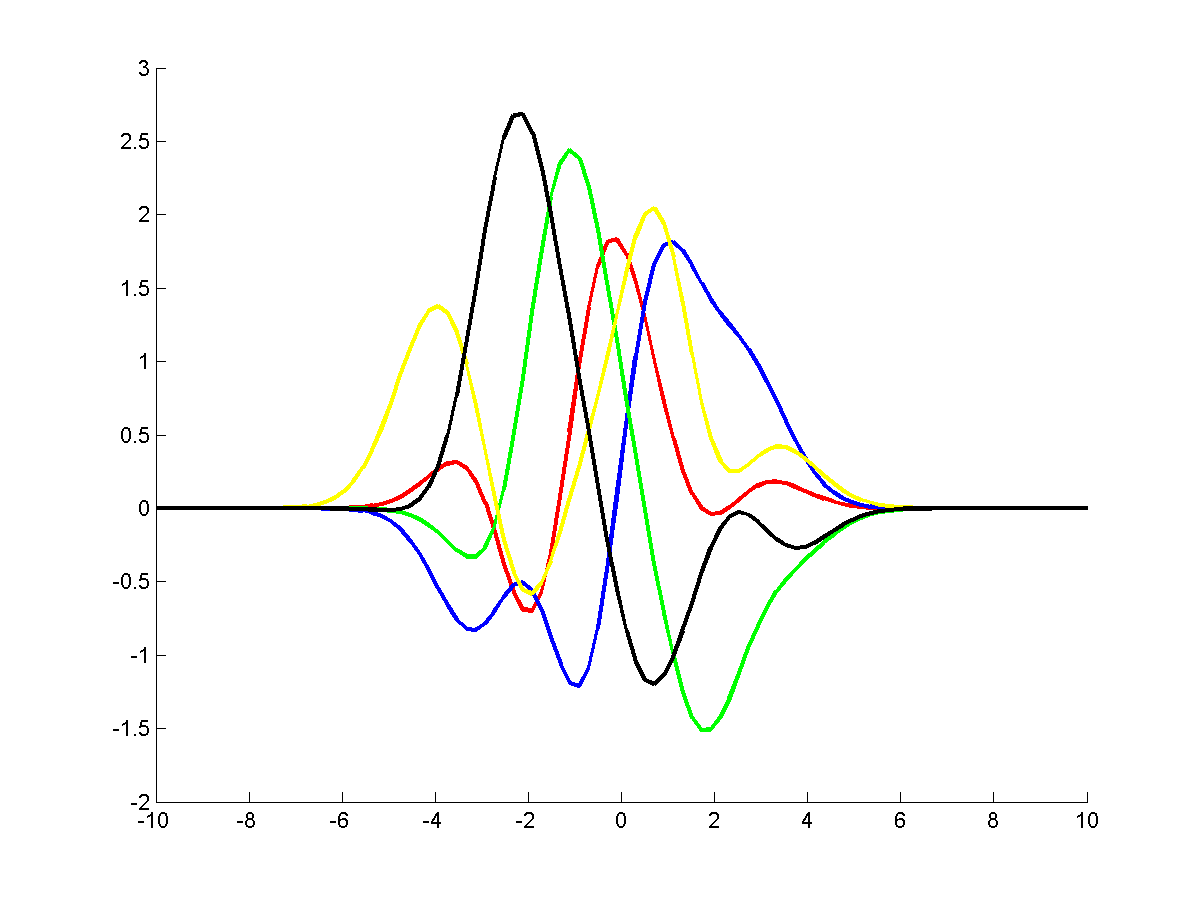
\includegraphics[trim=0cm 0cm 0cm 0cm, width=0.5\textwidth]{figures/plot1.png}%
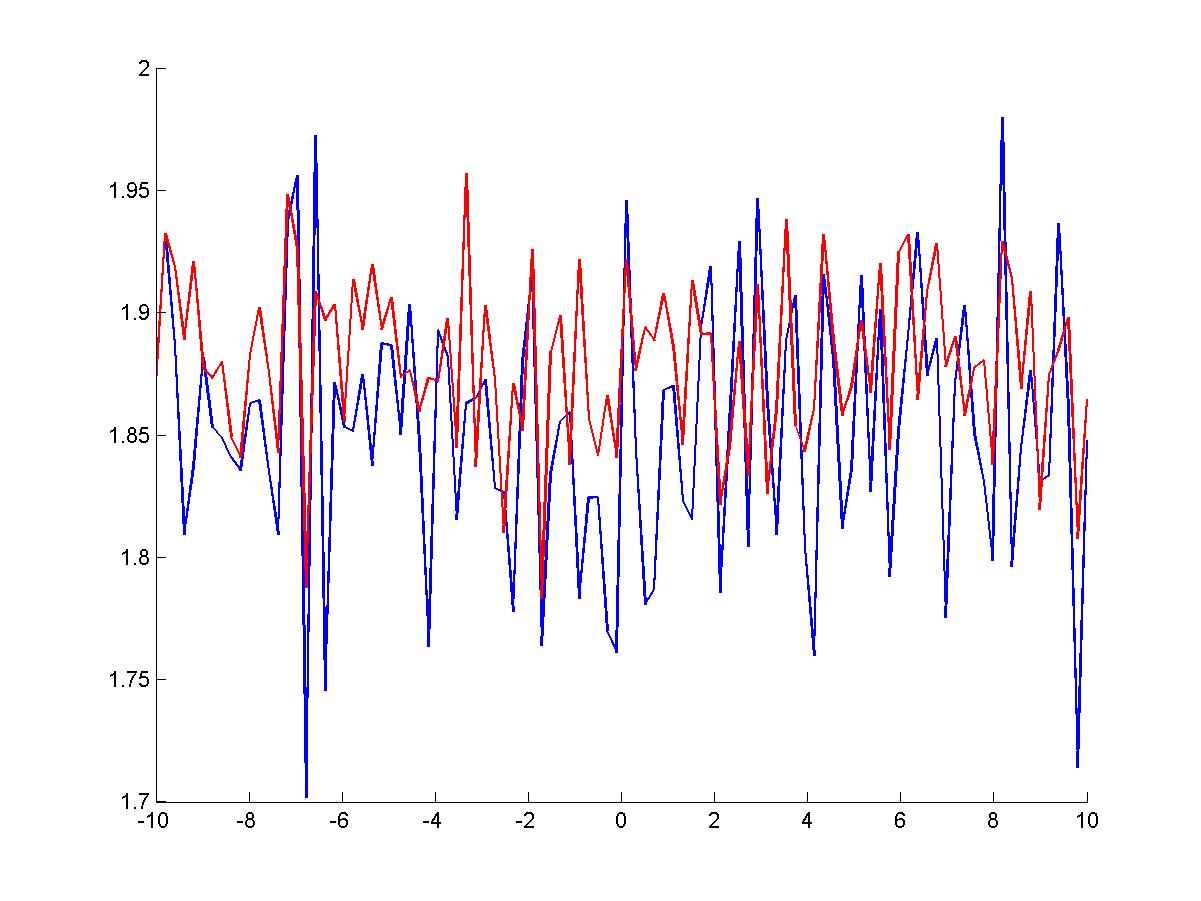
\includegraphics[trim=0cm 0cm 0cm 0cm, width=0.5\textwidth]{figures/plot2.png}
}
{\caption{\small{Functions drawn from {\GP} priors with {\SE} covariance functions. Lengthscales of 1.0 (left) and 20.0 (right) reflect the length of the trends the kernel is able to capture.  }}}
\end{figure}


\section{Gaussian Process Regression}

In the case of regression, we are modelling some function ${\f}$ given a set of $n$ noisy observations $ ({X}, \bm{y})$. Assume additive white noise, such that ${\mathbf{y}} = {\f} + \epsilon$, where $\epsilon \sim \mathcal{N}(0, \sigma_n^2)$. The likelihood, also known as the \emph{noise model}, becomes: 
\begin{equation*} \Pr ( \bm{y} \mid \f) =  \mathcal{N}( \f, \sigma_n^2 I) \end{equation*}
This likelihood function, together with the {\GP} prior, makes the task of predicting function values $\mathbf{f_T}$ for a set of test locations $X_t$ computationally feasible. The observations $(X, \bm{y})$ and the values of the function at test data locations have a joint Gaussian distribution \cite{rasmussen06}:
\begin{equation*} \Scale[0.95] { \left[ \begin{array}{c} \bm{y} \\ \bm{f_{*}} \end{array} \right] ~ \sim ~
 \mathcal{N} \left( \bm{0},  \left[ \begin{array}{cc} K(X, X) + \sigma_{n}^2 I & K(X, X_{*}) \\ K(X_{*}, X) & K(X_{*}, X_{*}) \end{array} \right] \right) ~ \triangleq ~
 \mathcal{N} \left( \bm{0},  \left[ \begin{array}{cc} K + \sigma_{n}^2 I & K_{*}  \\ K_{*}^\top & K_{T} \end{array} \right] \right) 
 }
\end{equation*}

For notational convenience, replace the covariances $K(X, X)$ and $K(X_{*}, X_{*})$ with $K$ and $K_{T}$, respectively. We also abbreviate the cross-covariance $K(X, X_{*})$ to $K_{*}$. By applying the standard formula for conditioning a joint Gaussian distribution \cite{rasmussenGPs}, we obtain the expression for the predictive distribution \cite{rasmussen06}: 

\begin{equation*} \mathbf{f_{*}} \mid X, \mathbf{y}, X_{*}  ~ \sim ~ \mathcal{N}\left( ~ K_{*}^{\top} ( K + \sigma_n^2I)^{-1} \mathbf{y} ~,~ K_{T} - K_{*}^{\top}( K + \sigma_n^2I)^{-1} K_{*}   ~ \right) \end{equation*}

The equation above shows the noise-free predictive mean and variance of the {\GP} at the test points $X_{*}$. To obtain the predictive distribution for $\mathbf{y_{*}}$, we just need to add $\sigma_n^2$ to the predictive variance in the equation above. $ K_{T} = K(X_{*}, X_{*}) $ is the prior covariance, from which we subtract the strictly positive term $K_{*}^{\top}( K + \sigma_n^2I)^{-1} K_{*}$ to obtain the covariance of the posterior distribution. This reduction in variance reflects the fact that conditioning on the data gave us additional information which reduced our uncertainty about the underlying function \cite{rasmussen06}. 

The complexity of the algorithm computing these values is $O(n^3)$: it is dominated by the inversion of $ K + \sigma_n^2I$. The Cholesky decomposition is typically used instead of inverting the matrix directly, as it has lower overhead and provides better numerical stability. Having computed the inverse, the costs of predicting the mean and the variance for a single test point $x_{*}$ are $O(n)$ and $O(n^2)$, respectively.  

% For the {\SE} kernel considered above, the lengthscale length also affects the shape posterior of the mean

\subsection{Learning the Hyperparameters}

The choice of adequate kernel hyperparameters is essential for adapting the covariance function to the data set provided. Popular machine learning models such as support vector machines or splines use cross-validation to learn hyperparameters. An advantage of Gaussian processes is that the higher values of the marginal likelihood reflect better models \cite{zoubinoccam, rasmussen06, rasmussenGPs}. Therefore, the `best' hyperparameters are those which maximise the marginal likelihood (also known as \emph{evidence}). 

In the regression setting, we can use the fact that $\bm{f} \mid X \sim \mathcal{N}(\bm{0}, K)$ and that $ \bm{y} \mid \bm{f} \sim \mathcal{N}(\bm{f},\sigma_n^2 I ) $ to conclude that $ \bm{y} \sim \mathcal{N}(\bm{0}, K + \sigma_n^2 I) $. Using this result, the (log) marginal likelihood can be expressed as:

\begin{equation*} L ~=~ \log \Pr ( \bm{y} \mid X)  ~=~  - \frac{1}{2} \bm{y}^{\top} (K + \sigma_n^2 I)^{-1} \bm{y} - \frac{1}{2} \log \left| K + \sigma_n^2 I \right| - \frac{n}{2} \log 2\pi \end{equation*} 
The first term in the equation above is a negative quadratic measuring how well the kernel fits the target values $\bm{y}$. The second term penalises overly complex models, ensuring that the marginal likelihood includes an automatic Occam's razor effect for achieving a trade-off between the quality of fit and predictive power on new data. This is important because the function learned could get arbitrarily close to the evidence by setting the signal variance $\sigma_n$ to $0$. That function would model the noise as part of the underlying signal, leading to poor predictive performance. The third term is a normalising constant which does not affect model selection. 

The automatic Occam's razor effect greatly simplifies the training process, as there are no parameters balancing model fit and model complexity to be set manually. Training a {\GP} reduces to finding the values of model hyperparameters which maximise the marginal likelihood given the observed data. Since we can find partial derivatives of the marginal likelihood with respect to the hyperparameters, we can use standard gradient based optimisation procedures such as conjugate descent \cite{rasmussenGPs}. As described in subsequent Chapters, this is usually a non-convex optimisation problem: different optima correspond to different interpretations of the data.  This means that the optimisation procedure should be re-run with different starting hyperparameters to avoid particularly bad local optima. 

%Prediction: http://mlg.eng.cam.ac.uk/tutorials/06/es.pdf around page 13

%Discuss the role of the covariance function... And show the difference between a lengthscale of 0.05 and 0.5, i.e. http://www.cs.toronto.edu/~hinton/csc2515/notes/gp_slides_fall08.pdf page 25. Page 34 of this tutorial also to be mentioned. 


\section{Gaussian Process Classification}

In binary classification, examples have two different labels: $y_i \in \{ -1, 1 \} $. There is no underlying real-valued function $\mathbf{f}$ to model. In order to tackle this problem using Gaussian processes, we will assume the existence of a \emph{latent function} $\mathbf{f}$ which governs the class membership of the data. To obtain the prior class distribution at test point $\mathbf{x_{*}}$, we convert the value of $\mathbf{f}$ at that point into a valid `{class 1}' probability using the \emph{response function} $\sigma$:

\begin{equation*} \pi(\mathbf{x_{*}}) \triangleq \Pr(y_{*} = +1 \mid \mathbf{x_{*}}) = \sigma(\mathbf{f}(\mathbf{x_{*}})) \end{equation*} %~~~ \mbox{and} ~~~  \Pr(y_{*} = -1 \mid {\bm{x_{*}}) = 1 - \sigma(\mathbf{f}(\bm{x_{*}}))  \end{equation*}


As the sigmoid function $\sigma$, we could use the logistic sigmoid $\sigma(x) = 1 / (1 + e^{-x})$ or the cumulative Gaussian distribution $\Phi(x)$. These functions `squash' their arguments, which can be arbitrary real numbers, to values between $0$ and $1$. As the output of $\mathbf{f(x)}$ can be an arbitrary real number, this step is required to give a valid probabilistic interpretation to the values given by the prior class distribution $\pi$. 

$\pi(\mathbf{x})$ represents our subjective belief that the example at $\mathbf{x}$ belongs to class 1. For binary classification, the probability of the other class is simply $1 - \pi(\mathbf{x})$. If we let $f_i = \mathbf{f}(x_i)$, we can concisely represent the likelihood (for a single example) as:
\begin{equation*} \Pr(y_i \mid x_i, \mathbf{f}) = \Pr(y_i \mid \mathbf{f}(x_i) )  = \sigma(y_i \mathbf{f}(x_i)) \triangleq \sigma (y_i f_i) \end{equation*} 
The multi-class version is harder, as the \emph{softmax function} replaces the sigmoid \cite{rasmussen06}. 

We are not particularly interested in the actual values of $\mathbf{f}(x_{*})$: we care only about the class membership of points at $x_{*}$. The latent function is there to act as the Gaussian prior to be integrated out when performing inference. The difficulty lies in the fact that the likelihood model is no longer Gaussian. If there are $n$ observed examples $\{ X, \mathbf{y} \} = \{ (\mathbf{x_i}, y_i), i \in 1, \ldots, n \} $, and we adopt the notation that $y_{i} = i$ for $i = \pm 1$, we can express the joint likelihood $\Pr(\mathbf{y}\mid\mathbf{f})$ as:
\begin{equation*} \displaystyle  \Pr(\mathbf{y}\mid\mathbf{f}) ~~=~~ \prod_{i = 1}^{n}{\Pr(y_i\mid{f_i})} ~~=~~ \prod_{i=1}^{n}{\sigma(y_i f_i)} \end{equation*}
If we assume a zero-mean $\GP(0, K)$ over the latent function $\mathbf{f}$ and let $\bm{\Sigma} = K(X, X)$, the posterior distribution of the latent function can be expressed as:
\begin{equation*}  \displaystyle  \Pr( \mathbf{f}  \mid X, \mathbf{y} ) = \frac{ \Pr(\mathbf{f} \mid X)  \Pr( \mathbf{y} \mid \mathbf{f}) }{\Pr(\mathbf{y} \mid X)}  =  
 \frac{ \mathcal{N}( \mathbf{f} \mid 0, \bm{\Sigma} ) }{ \Pr(\mathbf{y} \mid X) } \prod_{i=1}^{n}{\sigma(y_i f_i)}   \end{equation*}
This expression contains the marginal likelihood $\Pr(\mathbf{y} \mid X)$, which becomes: 
\begin{equation*} \displaystyle \Pr( \mathbf{y} \mid X  ) = \int{ \Pr ( \mathbf{y} \mid \mathbf{f} ) ~ \Pr( \mathbf{f} \mid X ) ~ \mathrm{d}\mathbf{f}  =  \int{  \left( \prod_{i=1}^{n}{\sigma(y_i f_i)} \right) \mathcal{N}( \mathbf{f} \mid 0, \bm{\Sigma} )  ~ \mathrm{d}\mathbf{f}  }}  \end{equation*}
The posterior and the marginal likelihood involve a product of a Gaussian with a product of sigmoid functions, which makes both of these expressions analytically intractable. The predictive distribution $ \Pr( \mathbf{y_{*}} = 1 \mid X, \mathbf{y}, x_{*})$ and the gradients of the marginal likelihood required to fit the model hyperparameters during the training process become intractable as well \cite{rasmussen06, gpcapprox, gpcinference}. 

This means one has to resort to approximations in order to perform classification using Gaussian Processes. Most of the known approaches revolve either around Markov chain Monte Carlo sampling or Gaussian approximations to the posterior distribution, such as Laplace's method or Expectation Propagation \cite{gpcinference}. % 

% http://papers.nips.cc/paper/2903-assessing-approximations-for-gaussian-process-classification.pdf IMPORTATNT
% http://mlg.eng.cam.ac.uk/tutorials/06/es.pdf slide 24
% http://people.ee.duke.edu/~lcarin/David1.27.06.pdf  rasmussen NIPS 2005 compares EP and Laplace. 
% http://homepages.inf.ed.ac.uk/ckiw/talks/nips06.pdf

\subsection{Approximative Inference for {\GP} Classification}

Markov chain Monte Carlo sampling methods can be used to obtain exact estimates of the required distributions. However, these estimates require very long running times to converge \cite{gpcapprox}. As such, they are less applicable in practice, but they provide a gold standard to compare the analytic approximations against. 

The analytic approximations such as Laplace's method or Expectation Propagation compute Gaussian approximations to the posterior $\mathbf{q}(\mathbf{f_{*}} \mid X, \mathbf{y}) = \mathcal{N}( \mathbf{f} \mid \mathbf{m}, \mathbf{A})$. The distribution of the latent function $\mathbf{f}_{*}$ at test point $x_{*}$ becomes:

\begin{equation*} \Pr(\mathbf{f_{*}} \mid X, y, x_{*}) \approx \mathbf{q}(\mathbf{f_{*}} \mid \mathbf{m}, \mathbf{A}) = \mathcal{N}(\mu_{*}, \sigma_{*}^{2})  \end{equation*}
\begin{equation*} \mu{*} = \mathbf{k_{*}^{\top} \mathbf{K^{-1}} \mathbf{m} ~~~ \mbox{and} ~~~ 
\sigma_{*}^{2} = k(x_{*}, k_{*}) - \mathbf{k_{*}^{\top}(\mathbf{K^{-1}} - \mathbf{K^{-1}AK^{-1}})\mathbf{k_{*}} } } \end{equation*}

$\mathbf{k_{*}}$ denotes the vector of prior covariances between the training data $X$ and $x_{*}$. $\mathbf{m}$ and $\mathbf{A}$ are parameters of the approximate posterior $\mathbf{q}$ to be learned using Laplace's method or Expectation Propagation \cite{gpcinference}. If we use the cumulative Gaussian distribution $\Phi$ as the sigmoid function, we can obtain an analytic expression for the predictive distribution as well:

\begin{equation*}  \displaystyle \mathbf{q}(y_{*} = 1 \mid X, \mathbf{y}, \mathbf{x_{*}} ) ~=~ \int{ \Phi(\mathbf{f_{*}}) ~ \mathcal{N}(\mathbf{ f_{*} } \mid \mu_{*}, \sigma_{*}^{2}) \mathrm{d}\mathbf{f_{*}}  ~=~ \Phi \left(\frac{\mu_{*}}{\sqrt{1+\sigma_{*}^{2}}}\right)   }    \end{equation*} 

\subsection{The Laplace Approximation}

Laplace's method finds the approximate value of the unnormalised log posterior by performing a second-order Taylor expansion around the mode of this distribution. The approximate log posterior at the test points can be expressed as:
\begin{equation*} \log \mathbf{q}(\mathbf{f} \mid X, \mathbf{y} ) \approx \log \mathbf{q}(\mathbf{m}) - \frac{1}{2} ( \mathbf{m} - \mathbf{f} )^{\top} \mathbf{A^{-1}} ( \mathbf{m} - \mathbf{f} ) \end{equation*}
\begin{equation*} \mbox{where~~} \displaystyle \mathbf{m} = \argmax_{f \in \mathbf{R^n}}{ \log{\mathbf{q}(\mathbf{f} \mid X, \mathbf{y})} }. \end{equation*} 

The likelihood and the prior are both log-concave and unimodal functions, which means $\mathbf{m}$ can be approximated using the iterative Newton-Raphson method:  
\begin{equation*} \mathbf{f} ~\gets~ \mathbf{f} ~-~ (~ \nabla \nabla_{\mathbf{f}} \log \mathbf{q}(\mathbf{f})~)^{-1} ~ \nabla_{\mathbf{f}} \log \mathbf{q}(\mathbf{f}))  )  \end{equation*}
This procedure usually converges to the mode within a few iterations. The covariance matrix of the approximate posterior distribution can be expressed as $ \mathbf{A} ~=~ \mathbf{\nabla \nabla_{\mathbf{f}} (\log \mathbf{q}(\mathbf{m}))^{-1}}$ \cite{gpcinference}. The closed-form expression for $ \mathbf{q}(\mathbf{f} \mid X, \mathbf{y} )$ can be used to obtain a closed-form approximation to the log marginal likelihood $\log \Pr(\mathbf{y} \mid X)$: 

\begin{equation*} \log \Pr(\mathbf{y} \mid X) ~\approx~ \log \mathbf{q}(\mathbf{y}\mid X) ~=~ \int{ \Pr(\mathbf{y} \mid \mathbf{f}) ~ \mathbf{q}(\mathbf{f} \mid X) ~ \mathrm{d}\mathbf{f} } ~ = \end{equation*}
\begin{equation*}  ~~~~~~~~~ = ~ \log \mathbf{q}(\mathbf{m}) ~+~ \frac{n}{2}\log(2\pi) ~+~ \frac{1}{2}\log |\mathbf{A}|  \end{equation*} 

The derivatives of the marginal likelihood with respect to the $\GP$ hyperparameters (omitted from all the expressions above) have closed-form solutions, so they can be used for hyperparameter optimisation \cite{gpcapprox}. 

\subsection{Expectation Propagation}

Expectation Propagation goes further than Laplace's method: the approximate posterior distribution constructed tries to match the first two moments of the actual distribution. The fundamental problem with Laplace's approximation is that the posterior mode becomes less representative of the posterior mean as the number of dimensions increases \cite{gpcapprox, gpcinference}. 

The probability mass is concentrated in a thin shell (far) away from the mode: the posterior mean moves towards this high density region, but the posterior mode stays closer to the origin. This means that Laplace's method produces overly cautious predictive distributions which are often inaccurate even near the training locations. As shown in previous work by Kuss and Rasmussen, EP tends to outperform Laplace's method on real-world data sets \cite{gpcapprox, gpcinference}. 


The two methods have the same asymptotic complexity, dominated by several iterations of matrix inversions which take $O(n^3)$ time. However, the computational overhead for Expectation Propagation is substantially higher, making Laplace's method {much} faster in practice. The difference in speed and performance between these two methods will be analysed in subsequent Chapters. 

\clearpage


\chapter{Related Work} 

In this chapter, I will present recent research on kernel learning and outline the ideas behind Additive Gaussian Processes and the work on kernel structure discovery for {\GP} regression, which was the main inspiration for this Research Project.  

\section{Kernel learning}

Nonparametric models can learn arbitrarily smooth functions from the training data. As the number of dimensions $D$ increases, the basic versions of these algorithms need to use very large data sets to extract the underlying structure. Even if such data sets are available, their size makes inference using nonparametric methods such as {\GP}s computationally infeasible. This means that \emph{additional constraints} on the structure of the models need to be imposed to make inference with high dimensional data sets possible. 

Generalised additive models (GAM) assume that the response function $y$ is a transformed sum of functions defined on individual dimensions. If $g$ is the \emph{link function} and $\mathrm{f_i}$ potentially different functions operating on different input dimensions, then:
\begin{equation*} g( y ) ~=~ \mathrm{f_{1}}(x_1) + \ldots + \mathrm{f_{D}}(x_D)  \end{equation*}
Even though this is a very strict constraint on the model structures permitted, the models constructed often perform well and are able to provide interpretability by directly showing the response function's dependence on each of the dimensions.  

The problem of constructing kernels using weighted sums of base kernels has been studied extensively \cite{christoudias2009bayesian}. Most of these algorithms find the optimal solution in polynomial time by specifying the component kernels and hyperparameters beforehand.  
Kernel methods, on the other hand, allow the response function to depend on all the input dimensions simultaneously: \begin{equation*} y ~=~ \mathrm{f}(x_1, \ldots, x_d)\end{equation*}
Examples of such methods include Gaussian Processes with Squared Exponential kernels. More specifically, the {\SE} Automatic Relevance Determination (ARD) kernel allows the input dimensions to vary across different dimensions, as opposed to the previously defined isotropic kernel. The {\SE} ARD kernel function is:

\begin{equation*} K(\mathbf{x}, \mathbf{x'}) ~=~ \sigma_0^2  \exp \left(  - \frac{1}{2} \sum_{i=1}^{d}\frac{({x_i}-{x_{i}'})^2}{{ {\lambda_{i}^2}}} \right) ~ \end{equation*} 

Other popular approaches learn kernel embeddings into low-dimensional spaces and use fixed kernel structures in those spaces \cite{lawrence2005probabilistic}. Deep neural networks have also been applied to learning embeddings \cite{salakhutdinov2008using}. Even though deep networks are not formally nonparametric models, they can express very flexible functions, as the number of units in their layers often exceeds the number of (hyper)parameters in traditional BNP models. The success of these approaches relies on inferring structure from the density $\Pr(x)$, so is most naturally applied to unsupervised learning problems. 

The work presented in this Dissertation builds on and extends previous research on automatic kernel construction for the purposes of classification. In this context, most of the interesting structure to be captured lies in $\mathrm{f(\mathbf{x})}$, making the methods geared towards unsupervised learning less relevant.

\section{Additive Gaussian Processes}

Duvenaud et al. (2011) generalise GAM and the {\GP}  {\SE} kernel models by constructing a {\GP} kernel which implicitly sums over \emph{all possible products} of one-dimensional base {\SE} kernels \cite{duvenaud2011additive11}. The \emph{additive kernels} which sum over all one-dimensional base kernels and over \emph{all products} of $n$ distinct base kernels are given by:
\begin{equation*} k_{1}(\mathbf{x, x'}) = \sigma_{1}^2  \sum_{i=1}^{D}{k_{i}(x_{i}, x_{i}')}  \mbox{~~~~and~~~~}  k_{n}(\mathbf{x, x'}) = \sigma_{n}^2  \sum_{1 \leq i_1 < \ldots i_n \leq D}{ \left[ \prod_{d=1}^{n}{k_{i,d}(x_{i_d}, x_{i_d}')} \right] }  \end{equation*}

The $n$th additive kernel $k_{n}$ represents the sum of all possible $n$-way interactions of the input dimensions. $\sigma_n$ represents the variance hyperparameter of each order of interaction. Unlike other approaches to kernel learning which require manual specification of the kernel structure, Additive {\GP}s only have to fix the $n$ functions $\mathrm{f_1 \ldots f_n}$ to be used as the basis functions for each of the dimensions. 

Each $k_n$ term contains $ {D \choose n} $ different product terms. The full additive {\GP} is defined as the sum of kernels for all possible orders of interaction: 
\begin{equation*} k_{\mathrm{full}}(\mathbf{x, x'}) = \sum_{i = 1}^{D}{ k_{i}(\mathbf{x, x'}) }  \end{equation*}

The full additive kernel includes any potential interaction between any number of basis functions. The model is very general: the $k_1$ summation represents the GAM model and the $k_{D}$ summation represents the {\GP} {\SE} ARD kernel. Its hyperparameters consist of the additive kernel variances $\sigma_1 \ldots \sigma_{D}$ and the hyperparameters of each of the $n$ basis functions (lengthscales, signal variances, etc). These can be learned by optimising the marginal likelihood of the training data \cite{duvenaud2011additive11}. 

The $\sigma_1 \ldots \sigma_n$ hyperparameters are very informative: they show what proportion of the target function's variance comes from each order of interaction. Low order interactions between different dimensions can be represented visually. First-order terms represent individual basis functions which we can plot after learning the hyperparameters. For two-way interactions, we can plot the posterior means of the individual second-order terms. For higher level terms, plotting the functions learned is not straightforward, and interpreting the higher level interactions between features becomes increasingly hard.  


If we consider all interactions of order up to $n$, the Additive {\GP} contains $O(2^n)$ terms. For $n \coloneqq D$ the summation would be intractable if approached naively. It is possible to reduce the time complexity to $O(D^2)$ using the Newton-Girard formulae for computing \emph{elementary symmetric polynomials}. This makes the procedure for training and using additive {\GP}s tractable. Low-level interactions prove to be the most relevant for modelling and providing interpretability. This means one can trade small loses in predictive accuracy for substantial improvements in speed while retaining the interpretable components of the additive kernel \cite{duvenaud2011additive11}. 

Additive GPs are applicable to both classification and regression problems. Standard {\SE} and GAM kernels fail to capture structure which involves patterns longer than the lengthscales of the kernels they use. Additive {\GP}s are able to capture non-local structure using the higher-order interactions and use this information for  extrapolation to distant parts of the input space \cite{duvenaud2011additive11}. 

Additive {\GP}s have been compared to GAM models, {\GP} {\SE} models, Linear and Logistic regression, as well as to other state of the art methods such as Hierarchical Kernel Learning (HKL). In the cases when the data was explained mostly by low-order interactions, Additive {\GP}s outperformed the other methods. When the higher levels of interactions were more dominant, the performance of Additive {\GP}s resembled that of the {\GP} {\SE} model, which makes sense since these kernels represent a subset of the kernels included in the full Additive {\GP} model. 


\section{Kernel structure discovery for GP regression}

In spite of the growing popularity of nonparametric Bayesian methods, the choice of kernels is still left to the individual user. This is a major obstacle to making these models easily accessible to non-practitioners without a machine learning background. Additive {\GP}s remove the need for the users to specify the exact kernel structure or its hyperparameters. This model requires manual specification of the basis kernels to make the full kernel construction automatic. Setting these functions requires expert knowledge, so the next step in automatizing kernel construction is to eliminate the need for users to choose the basis kernels themselves. 

Duvenaud, Lloyd et al. (2013) tackle this problem by defining a \emph{grammar} over the kernel structures \cite{duvenaud13}. The base kernels of this grammar are one-dimensional kernels defined on each of the input dimensions, such as $\SE_1$, $\RQ_2$, $\Per_3$, where the subscript indicates the dimension the given base kernel applies to. In the original work, four kernel families are considered: $\SE$, $\RQ$, $\Lin$ and $\Per$. Subsequent work includes the changepoint kernel as well \cite{lloyd14}. Any algebraic expression which combines these kernels using the $+$ and $\times$ operators defines a valid kernel structure. 

This grammar includes all models which can be expressed using Additive {\GP}s, GAM and {\SE} models. It can also express other models such as $ \SE_1  \times (\SE_3 + \SE_4)$. This kernel is not equivalent to $\SE_1 \times \SE_3 + \SE_1 \times \SE_4$: the first model has three, and the second model has four lengthscale hyperparameters.  

Next, we need to define the procedure which explores this grammar to find the best composite kernel for the given data set. The search procedure starts by evaluating all one-dimensional base kernels and assigning them a \emph{score value}. 

Marginal likelihood is used as the model selection criterion. Since we are comparing kernel families defined by composite kernels, we need to integrate out the model hyperparameters. This integral is intractable and is approximated by the Bayesian Information Criterion, which penalises models that overfit by introducing too many hyperparameters, in this case corresponding to large numbers of kernels \cite{schwarz1978estimating}.  

Once the kernel structure (corresponding to some expression $\mathcal{A}$) with the best BIC value is identified, the search expands this structure by trying to add or multiply each of its subexpressions $\mathcal{S}$ with all base kernels $\mathcal{B'}$. The procedure also tries to replace any base kernel $\mathcal{B}$ in $\mathcal{A}$ with any other base kernel $\mathcal{B'}$. Of all the kernel structures constructed, the one with the best BIC value is chosen as the next kernel to expand. This process is repeated until the search can no longer improve on the best BIC value by using a more sophisticated kernel structure. 

% The specification of these functions still requires that the user possesses some expert knowledge. 
The Additive {\GP} model implicitly sums over an enormous number of kernels. In most cases, few kernels (often low-order interactions) account for most of the contribution to the latent function. This means that a much `lighter' model can often be used in place of the Additive {\GP} model. Indeed, {\GP} Structure Search is able to outperform the {\GP} Additive model using much smaller kernels which at the same decompose into easily interpretable components \cite{duvenaud13, lloyd14}. %, especially if all the base function interactions found are first or second-order, making them easy to visualise. 

This method provides a data-driven method to choose the kernel structure for any specific problem. The space of kernels that the search can construct is extremely rich, and there is no manual parameter tuning on the side of the user. In spite of the very general kernel grammar, the use of the BIC approximation for model selection raises important questions about the validity of this procedure. Devising a well-founded guiding criterion would be a major step in dispelling the existing skepticism about the potential of this automatic kernel discovery procedure. 

%Moreover, the complexity of the search is exponential, as the number of potential kernels to evaluate grows exponentially as the search depth increases. 

{\GP} Structure Search for regression achieved formidable results, and the subsequent work on automatic report generation has attracted a lot of interest in the research community. The main goal of this Research Project was to investigate whether automatic kernel construction is possible for classification problems as well. 

% Unsupervised structure discovery - mention that paper, maybe initially, as similar work... 
%- define a grammar, write out a couple of kernel expressions one is able to construct using this search. 
%- data-driven approach to choosing kernel structures automatically can help make nonparametric regression and classication methods accessible to non-experts
%- shows how the composite kernel structure relates to the underlying patterns in the data, thus providing interpretability. 

%- greedy search over the defined kernel space. At each stage, picks the highest scoring kernel and expands it by applying all possible operators.

\clearpage

\chapter{Kernel Structure Discovery for GP Classification} 


This chapter presents the work done on extending the kernel structure search procedure to the classification case. It first discusses the algorithm and the design choices involved in developing for performing kernel structure discovery in these problems. It provides a proof of concept for the algorithm by demonstrating that it is able to uncover the underlying true kernel for synthetic data sets. The last part of this Chapter deals with applying the search procedure to real-world data sets and discusses the difficulties overcome in achieving state of the art performance. 

% We will then show that this approach is able to extract the underlying truth in synthetic data sets. I will then analyse its performance on real world data sets.

\subsection*{The Difficulties with Classification}

In the classification setting, the likelihood functions become non-Gaussian and the binary data labels decrease the information content of the data sets. Finding interpretable components and patterns in the data becomes much harder than in the case of the time series data sets considered in the existing work on regression. Finally, the use of the Bayesian Information Criterion as a model selection criterion becomes even more problematic, as the number of effective hyperparameters becomes harder to estimate in the classification setting. 

\section{Building the Models}

This section presents the kernel grammar chosen and the search operators used to define it. Three different methods for performing approximative inference are analysed and the implementation details of the hyperparameter estimation are discussed.  

\subsection{Defining the Kernel Grammar}

Adding or multiplying with a base kernel. Discuss what adding two kernels or multiplying them accomplishes. Show SE1, SE2, individual plots, then SE1 + SE2, SE1 X SE2 plots.

Compare with the regression case, explain why the RQ and Periodic kernel make less sense, and justify why a pure {\SE} grammar was used (together with a constant mean function to deal with class imbalance in the data sets).  

Discuss sum of products vs grammar which can express everything. The grammar can represent exactly the terms in an Additive {\GP} with all base functions set to {\SE}s.
Sum of products achieves lower accuracy, but makes the search much faster and the composite kernels much more interpretable. 

Should I include (and how much) implementation details: languages used, parallelisation on fear, details of GPML and the infrastructure of the system built...

\subsection{Approximative Inference}
%\subsection{Learning the Hyperparameters}

EP vs Laplace vs VB in GPML. EP much slower than Laplace, difference in performance non-existant in all experiments: pure {\SE} grammar makes hyperparameter fitting much easier than was the case in previous work on regression. VB bug?

Reiterate that marginal likelihood is used as the criterion for model selection. Explain that the hyperparameters are found using conjugate gradients in GPML- quickly explain this procedure. 

Discuss the computational complexity: suited to use of small training sets, as the training complexity is $O(n^3)$. With larger data sets, we can still fit the hyperparameters faster using subsampling, and this will be heavily exploited in subsequent work, but the final fitting steps take $O(n^3)$ and as such prevent usage of very large data sets available today. 

Subsampling the training data to make the hyperparameter fitting faster: perform 300 iterations (a good rough guideline is the number of hyperparameters * 50) with 250 points randomly sampled from the data set, then perform an additional 50 iterations with the full data set. 

Due to the smoothness of the $\SE$ kernels, this algorithm converges to the same hyperparameters as the minimization that uses the entire data set for the whole process. 

Discuss parallelisation and the use of the cluster. Discuss and add a table of running times and numbers of restarts performed. 

\section{Searching for the Model}

Discuss the greedy search and backtracking, as well as feature reduction (all implemented). 

\subsection{Bayesian and Akaike Information Criteria}

%critique: Discuss different information criteria, i.e. the fact that RQs can be penalised more than an SE... preferring products to additive components, say that this is something we evaluate thoroughly and try to improve on. 

For high values of the number of data points $n$, the Bayesian Information Criterion can be approximated using the following expression:

\begin{equation*} BIC =  - 2 \ln L + k  \ln(n)  \end{equation*}

where $L$ is the log marginal likelihood of model $M$ on the data set $\mathbf{X}$: $\Pr(\mathbf{X} \mid \theta, M)$, where the hyperparameters $\theta$ are set to achieve the maximal value of $L$ using conjugate descent. $k$ is the number of \emph{effective hyperparameters} 
of the model: estimating this number is non-trivial, and a significant portion of our work consisted of examining different approaches to approximating this figure. 

The Akaike Information Criterion (AIC) penalises the number of parameters less than BIC does, no longer taking into account the actual size of the data set: 

\begin{equation*} AIC = - 2 \ ln L + 2 k \end{equation*}


\subsection{The Number of Effective Hyperparameters}
% ... i.e. the BIC Light section.

A major problem for applying BIC to classification is that estimating the number of effective hyperparameters is hard: not all of them affect the classification boundary equally. The only thing important for classification is the zero-crossings of the function (where it is greater, and where it is smaller than 0, for the purposes of prediction). Hence, smaller lengthscales are the most important factor, as they determine where the predictive mean's zero-crossings exactly are. Very large lengthscales equate to multiplication with constant functions, so they have less impact on the classification boundary. Signal variances are useful for computing the predictive variances and determining the relative contribution of each term, but only the predictive means matter for determining the target label. Not counting signal frequencies adds a quick boost to the quality of BIC as a model discriminator: we will refer to this `modified' criterion as \emph{BIC light}. 


\subsection{Cross-validated Training Accuracy}

Discuss the use of cross-validated train accuracy - how it may be expected to provide us with the ceiling performance, but in the end it doesn't improve much on BIC light and likMix models. 

Include algorithmic package pseudo code to explain the process. 

Show traces of the search, showing how it can build more and more complex models by achieving minimal gains in the marginal likelihood, oscillating around the same levels of performance and requiring many steps of the search to halt as there is no penalisation term for large composite models. Discuss stopping criteria (change in BIC smaller than some threshold). 

Explain that the reason that it can improve marginal likelihood by adding these irrelevant components is that multiplying by these allows the optimisation procedure to move out of the region where its stuck. Also, numerical instability due to use of approximations to the posterior may contribute to this behaviour.


%In this section, we consider the results achieved by the structure discovery procedure presented in the previous section. We first provide a proof of concept for the structure search procedure based on the BIC light search criterion: we will  show that it is able to extract correct kernel structure from synthetic data drawn from {\GP} priors with {\SE} kernels. then proceed to demonstrate that the performance of the procedure on real world data sets is on par with other state of the art methods such as additive Gaussian Processes and Random Forests. % Finally, we present the kernel decompositions on the real world data sets which can be used to uncover and visualise the underlying data patterns which dictate class membership of the data points. 

\clearpage

\section{Experiments with Synthetic Data}

To prove that the greedy structure search procedure is able to extract structure from data, the algorithm was first applied to data drawn from a single \gp{} prior. If the greedy search based on any of the three information criteria has potential, the procedure should be able to recover the original kernel given enough synthetic data. 

The amount of data available to the procedure, as well as the signal-to-noise ratio in the data were varied across experiments. As we decrease the noise levels and add more data points, the structure search should get closer to the underlying truth, that is the original kernel used to generate the data. Signal to noise ratio values of 100 and 1 correspond to white noise of magnitudes equal to 10\% and 100\% of the signal magnitude. The search results shown below used \emph{BIC light} as the guiding criterion: the correctly identified kernel structures are shown in bold.   ~~~~~~~~~~~~~~~~~~~~~~~~~~~~~~~~~~

\begin{table}[h]

\label{tbl:synthetic}
\begin{center}

\makebox[(\textwidth) ]{

\small 
\begin{tabular}{|c |  c |  c | c | }
\hline 
{True Kernel} & { N } & { Kernel recovered (SNR = 1) } &  { Kernel recovered (SNR = 100) }  \\ \hline

&100&  $\bm{[1]}$ &$\bm{[1]}$ \\
$\bm{[1]} $ & 300& $\bm{[1]}$ &$\bm{[1]}$ \\
\emph{3 dimensions}& 500& $\bm{[1]}$ &$\bm{[1]}$ \\ \hline


&100& ${[2]}$ &${[2]}$ \\
$\bm{{[2]} + {[2]} + {[2]}} $& 300& ${[2]}$ &${[2] + [2]}$ \\
\emph{3 dimensions}& 500& ${[2]}$ &${[2]} + {[2]}$ \\ \hline


 &100& $\bm{[2\times 3]} $ &$\bm{[2 \times 3]}$ \\
$\bm{[2\times 3]} $& 300& $\bm{[2\times 3]} $ &$\bm{[2\times 3]} $ \\
\emph{3 dimensions}& 500& $\bm{[2\times 3]} $ &$\bm{[2\times 3]} $ \\ \hline


&100& ${[1] + [4]}$ &$ { {[1]} + {[2]} + {[4]} }$ \\
$ \bm { {[1]} + {[2\times 3]} + {[4]} } $ & 300& $ {[1 \times 4]} +  {[2\times 3]} $ &$\bm{{[1]} + {[2\times 3]} + {[4]}}$ \\
\emph{4 dimensions}& 500& ${ {[1 \times 4]} + {[2\times 3]} }$ &$ \bm{ {[1]} + {[2\times 3]} + {[4]}}$ \\ \hline


&100& ${[1]} + {[4]}$ &${[1]} + {[2]}  + {[4]}$ \\
$\bm{{[1]} + {[2\times 3]} + {[4]} }$ & 300& ${[1\times 4]} + {[2\times 3]} $  &$\bm{{[1]} + {[2\times 3]} + {[4]}}$ \\
\emph{10 dimensions}& 500& ${[1\times 4]} + {[2\times 3]} $ &$\bm{{[1]} + {[2\times 3]} + {[4]}}$ \\ \hline


 &100& ${[4]} + {[5]}$ &$ {[1\times 9]} + {[4]} $ \\
$\bm{{[1]} + {[2\times 3]}  + {[4]} + {[5\times 6]} } $ & 300& ${[1]} + {[2]} + {[4]} + {[5\times 6\times 7]} $  & ${[1]} + {[1\times5\times6]}  + {[2\times3]} + {[4]}$  \\
\emph{10 dimensions}& 500& ${[1]} + {[1\times 4]} + {[2\times 3]} + {[5\times 6]} $  &${[1]} + {[1\times4\times5\times6]} + {[2\times3]} + {[4]}$  \\ \hline


&100& ${{[4\times7]}} $ & $\bm{{[3 \times 5 \times 7]}}$ \\
$\bm{{[3\times5\times7]}} $ & 300& ${{[2 \times  3 \times5\times7]}}$ &$\bm{{[3\times5\times7]}}$ \\
\emph{10 dimensions}& 500& ${{[2 \times 3\times5\times7]}}$ &$\bm{{[3\times5\times7]}}$ \\ \hline


 &100& ${[1\times3]} + {[10]}$  &${[1\times10]} $ \\
$\bm{{[1]} + {[3\times5\times7]}  +  {[10]}} $ & 300& ${[1]} + {[10]} $ &${[1]} + {[1\times10]} + {[3\times5\times7]}$  \\
\emph{10 dimensions}& 500& ${[1]} + {[10]}$ &$\bm{{[1]} + {[3\times5\times7]} + {[10]}}$  \\ \hline


&100& ${[3 \times 7]}$ &${[1]} + {[7\times9]}$ \\
$\bm{{[3\times5\times7\times9]}} $ & 300& ${[7\times9]}$ &$\bm{{[3\times5\times7\times9]}}$ \\
\emph{10 dimensions}& 500& $\bm{{[3\times5\times7\times9]}}$ &$\bm{{[3\times5\times7\times9]}}$ \\ \hline


 &100& ${[9 + 10]}$ &${[10]} $ \\
$\bm{ {[1]} + {[3\times 5\times 7\times 9]}  + {[10]} }$  & 300& ${[1]} + {[10]}$  &${[1 \times 5] + [7] + [10]}$ \\
\emph{10 dimensions} & 500& ${[1]} + {[3\times5\times9]} + {[10]}$  & $\bm{{[1]} + {[3\times5\times7\times9]} + {[10]}}$  \\
 
\hline
\end{tabular}
}     

 \end{center}

\end{table}

Kernel optimal rates give a bound on the performance of the structure search: on average, the search is (by design) unable to construct kernels that have better predictive performance than the one used to generate the data. The function optimal rates give a theoretical limit on what any model could achieve, as they compare the actual function (its values before adding noise) to the data after the noise is added. As a result, kernel rates are always below the function rates. The models constructed can achieve higher accuracy than either of these by chance, but are \emph{on average} inferior to both the kernel and the function optimal rates. 

\begin{table}[h]

\label{tbl:synthetic2}
\begin{center}

\makebox[(\textwidth) ]{

\small 
\begin{tabular}{|c |  c | c | r c  | c | c c | }
\hline
\multicolumn{2}{|c|}{  } & \multicolumn{3}{c|}{ SNR = 1 }  &  \multicolumn{3}{c|}{ SNR = 100 }   \\ \hline
{True Kernel} & { N } & Test Accuracy & Kernel &  Function & Test Accuracy & Kernel & Function \\ \hline

&100& \textbf{81.0\%} &  80.0\% & & \textbf{98.0}\% & 97.0\% &  \\
 $\bm{[1]} $ & 300& \textbf{82.7}\% & 82.0\% & 83.6\%  & \textbf{99.3\%} & 98.7\%  &  99.0\%   \\
\emph{3 dimensions}& 500 &   83.6\% & 83.8\% &  &  \textbf{98.4\%} & 98.4\% & \\ \hline


&100&   74.0\% & 	75.0\% & & 	\textbf{98.0\%} & 	98.0\% & \\ 
$\bm{{[2]} + {[2]} + {[2]}} $ & 300 &   \textbf{77.3\%} & 	77.0\% & 78.2\%	  &	\textbf{98.7\%} &  {98.7\%} & 98.8 \% \\
\emph{3 dimensions}& 500 &  \textbf{78.2\%} & 	78.2\% & &	\textbf{98.6\%} & 	98.6\% & \\   \hline


 &100 & 67.0\% & 68.0\% & 	& \textbf{89.0\%}  & 89.0\% & \\ 
$\bm{[2\times 3]} $& 300 & 69.7\% & 70.3\% & 74.8\%	& \textbf{94.7\%}  & 91.3\% & 98.0 \% \\ 
\emph{3 dimensions}& 500 & 71.4\% & 72.6\% & 	& \textbf{95.8\%}  & 93.4\% & \\  \hline


&100&  71.0\% & 80.0\% & & 82.0\% & 87.0\% & \\ 
$ \bm { {[1]} + {[2\times 3]} + {[4]} } $ & 300 & 73.0\% & 76.3\% & 76.4\% & \textbf{94.7\%} & 91.7\% & 97.4\% \\ 
\emph{3 dimensions}& 500 & 73.4\% & 74.8\% & & \textbf{94.2\%} & 91.8\% & \\  \hline

&100&  71.0\% & 80.0\% & & 82.0\% & 87.0\% & \\ 
$ \bm { {[1]} + {[2\times 3]} + {[4]} } $ & 300 & 73.0\% & 76.3\% & 76.4\% & \textbf{94.7\%} & 91.7\% & 97.4\% \\ 
\emph{10 dimensions}& 500 & 73.4\% & 74.8\% & & \textbf{94.2\%} & 91.8\% & \\  \hline


 &100 & \textbf{61.0\%} & 	60.0\% & 	 &  70.0\% & 	84.0\% & \\ 
$\bm{{[1]} + {[2\times 3]} + {[4]} + {[5\times 6]}  } $ & 300 & 67.7\% & 	70.7\% &  76.6\% &  91.0\% & 	92.3\% & 97.2\% \\ 
\emph{10 dimensions}& 500 & \textbf{73.4\%} & 	73.0\% & 	 &  \textbf{94.0\%} & 	92.0\% &  \\  \hline


%&100 & 68.0\% & 67.0\% & 79.0\% & 84.0\% \\ 
%$\bm{{[3\times5\times7]}} $ & 300 & 66.0\% & 	67.7\% & 89.0\% & 89.7\% \\ 
%\emph{10 dimensions}& 500 & 71.8\% & 69.4\%  & 91.4\% & 91.0\% \\  \hline
&100 &  53.0\% & 64.0\% & & \textbf{87.0\%} & 83.0\% &  \\ 
$\bm{{[3\times5\times7]}} $ & 300 & 69.3\% & 71.0\% & 79.0\% & \textbf{92.7\%} & 89.0\% & 98.4\%  \\ 
\emph{10 dimensions}& 500 & {73.2\%} & 73.6\% & & \textbf{93.6\%} & 91.6\% &  \\    \hline


 &100 & \textbf{71.0\%}  & 70.0\% & 	& 87.0\% & 92.0\% & \\  
$\bm{{[1]} + {[3\times5\times7]}  +  {[10]}} $ & 300 & \textbf{73.0\%}  & 71.3\% & 75.0\% & \textbf{94.3\%} & 94.3\% & 97.6\% \\ 
\emph{10 dimensions}& 500 &  70.0\%  & 72.2\% & 	& \textbf{93.8\%} & 92.8\% & \\ \hline


&100 & 57.0\% & 59.0\% &  &	65.0\% & 77.0\% & \\ 
$\bm{{[3\times5\times7\times9]}} $ & 300 & 59.3\% & 70.3\% & 77.0\% &    \textbf{83.7\%} & 82.7\% & 97.0 \% \\ 
\emph{10 dimensions}& 500 & \textbf{71.0\%} & 	69.0\% & & \textbf{85.6\%} & 82.6\% & \\   \hline


 &100 & 68.0\% & 74.0\% &  & 77.0\% & 	81.0\% &  \\ 
$\bm{ {[1]} + {[3\times 5\times 7\times 9]}  + {[10]} }$  & 300 & 70.7\% & 73.3\% & 78.2\% & 81.7\% & 89.0\% &  96.8\% \\ 
\emph{10 dimensions} & 500 & 72.0\% & 72.4\% &  & \textbf{90.6\%} & 	89.8\% &  \\ 
 
\hline
\end{tabular}
}     

 \end{center}

\end{table}

Commentary on these results. 


\clearpage

\section{Structure Discovery for Real-world Data Sets}

Describe the data sets first? Table of name, dimensionality, sample size. 

\subsection{Overfitting}

Dealing with very small and very large hyperparameters. Discuss what large ones mean (inconsequential for classification boundary) and what small ones do (overfitting). Explain how we set the minimal allowed lengthscale for each dimension and how discretised data presents a challenge. 

Overfitting with large lengthscales is to be expected, so we plot the histogram of accuracies for training and testing data when doing ten fold cross validation (with many different splits, i.e. seeds). From the plots below, we see that testing accuracy is expected to vary
when doing ten-fold cross validation with this amount of data. With 100 different splits (that is 1000 different data points), the training accuracy ranges from $59\%$ to $66\%$, while the test accuracy varies from $40\%$ to $90\%$, showing that the overfitting (or surprisingly 
good performance we encounter on some folds) is a something to be expected. 

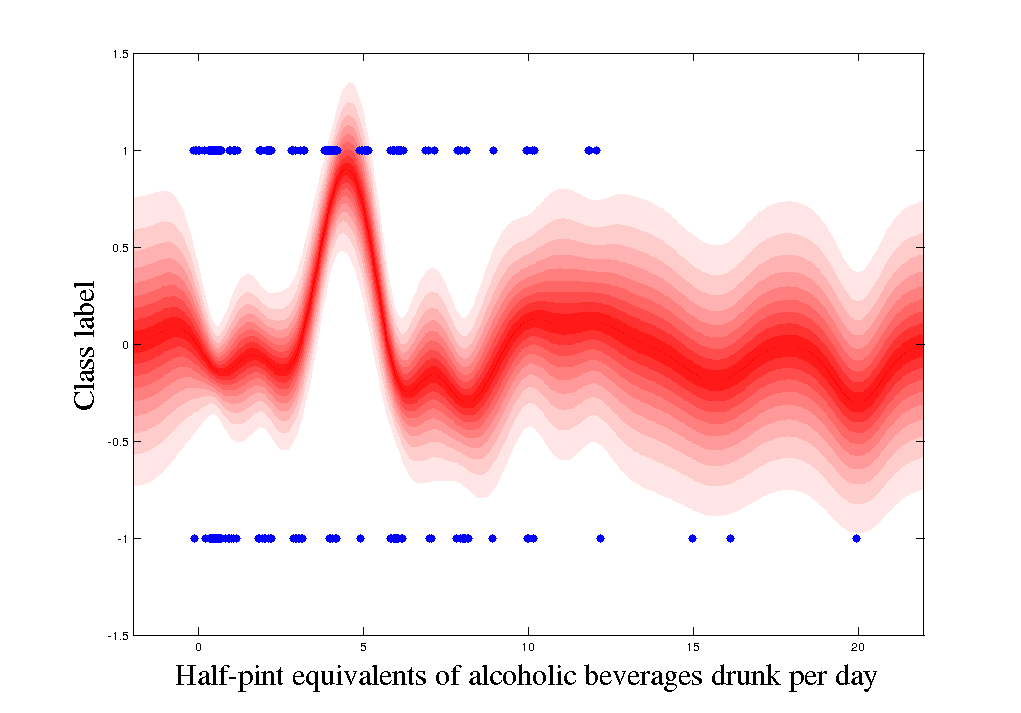
\includegraphics[trim=2cm 0cm 1cm 0cm, width=1\textwidth] {figures/liversmalllengthscale.png}


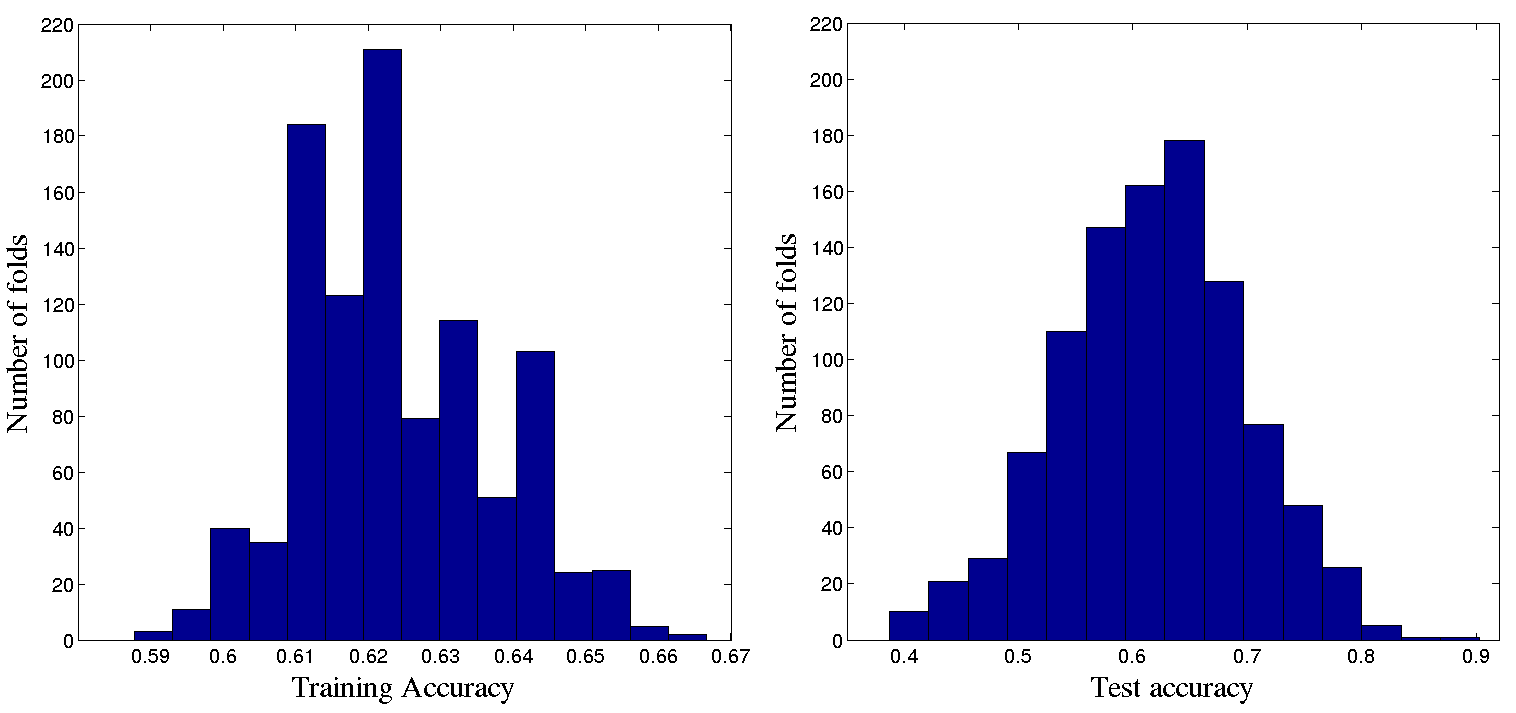
\includegraphics[trim=2cm 0cm 1cm 1cm, width=1\textwidth] {figures/overfitwithlargelength.png}

%Rasmussen paper explanataion of marginal likelihood GP behaviour:

The number of search steps figure that shows the level of overfitting (defined as the difference between training and testing accuracy) of the three metrics at different search stages across all the experiments on real-world data (discussed in later parts of the chapter) is shown below:  \\

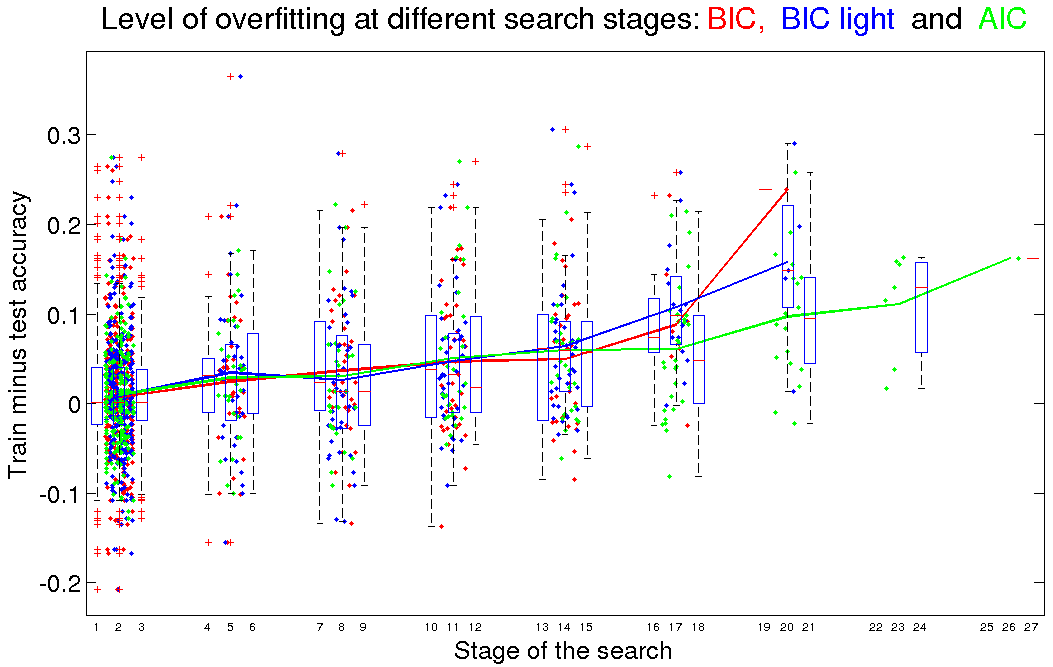
\includegraphics[scale=0.37]{figures/measureoverfit.png}

\clearpage

\subsection{Predictive Performance}

In this section, we compare the performance of models constructed using our algorithm with related methods and show that the performance of our structurally simpler models is on par with more complicated models such as Additive {\GP}s and Hierarchical Kernel Learning. 

We also compare the performance of structure search using different information criteria (BIC, AIC, BIClight), as well as the search guided by cross-validated training accuracy. We also show the performance of the model constructed using the alternative likelihood function. 


In addition to the structure search, we show the performance of the random forest method, which constructs 1000 decision trees using the training data and then uses the mode of the classifications produced by these trees to label the test set data. This method was intended to be a \emph{ceiling}
performance for our methods, as its focus is just predictive performance: it does not contribute to interpretability or our understanding of the data set considered. 


The table below contains the mean classication error across 10 train-test splits between different methods. The model with the best performance is shown in bold, together with all the other models whose predictions were not significantly different from those made by the best model. Statistical significance was determined using the \emph{paired t-test}. 

\begin{table}[h!]
\caption{{\small
Classification Percent Error
}}
\label{tbl:Classification Percent Error}
\begin{center}
\begin{tabular}{| l | r r r r | }

\hline Method & \rotatebox{0}{ breast }  & \rotatebox{0}{ pima }  & \rotatebox{0}{ liver }  & \rotatebox{0}{ heart }  \\ \hline
Logistic Regression & $7.611$ & $24.392$  & $45.060$ & \emph{ \textbf{{16.082}}} \\
GP GAM & \emph{\textbf{5.189}} & \emph{\textbf{22.419}}  & \emph{ \textbf{29.842}} & \emph{\textbf{16.839}} \\
HKL & \emph{ \textbf{5.377}} & $24.261$  & \emph{ \textbf{27.270}} & \emph{ \textbf{18.975}} \\
GP Squared-exp & \emph{ \textbf{4.734}} & \emph{ \textbf{23.722}}  & \emph{ \textbf{31.237}} & \emph{ \textbf{20.642}} \\
GP Additive & \emph{ \textbf{5.566}} & \emph{ \textbf{23.076}}  & \emph{ \textbf{30.060}} & \emph{ \textbf{18.496}} \\ \hline 
GPSS (AIC) & ${ 6.430 }$ & $\mathbf{22.529}$  & $ {28.924}$ & $ 19.860 $ \\
GPSS (BIC) & $ { 5.980 }$ & ${23.440}$  & $ {37.010}$ & $ \mathbf{18.150} $ \\
GPSS (BIC light) & $ { 6.430 }$ & $\mathbf{ 22.270 }$  & $ \mathbf{27.500} $ & $ \mathbf{17.820} $ \\
%GPSS (likMix) & $ \mathbf{ 11.240 }$ & $\mathbf{ 23.180 }$  & $ \mathbf{28.370} $ & $ \mathbf{16.460} $ \\
GPSS (crossValGuide) & $ \mathbf{ 5.090 }$ & ${ 23.700  }$  &  -  & $ \mathbf{17.160} $ \\ \hline
Random Forest & $ \mathbf{4.220} $ &  $ \mathbf{23.440} $ & $ \mathbf{24.030} $ &  $ \mathbf{17.130} $ \\ \hline
\end{tabular}
\end{center}
\end{table}

The paired t-test is tolerant of complete outliers: if a model is on par with the best model on 9 out of 10 folds and it performs badly on the 10th fold, this case is treated as an outlier and discarded.  
%This is the reason why the likelihood mixture model, which is clearly inferior to all other models on the breast data set, is still deemed to be on par with Random Forest and the CrossVal guided algorithm. 
This is why the BIC guided algorithm is deemed worse than Random Forest on the Pima dataset in spite of having the same average error. BIC is consistently worse than BIC light (the best model) whereas Random Forest manages to outperform BIC light on some of the folds. 



\chapter{Advancing the Automated Statistician}

\section{The Alternative Likelihood Function}

\subsection{Dealing with Outliers}

The reason that GPs out of the box are easily outperformed by classification specific schemes such as SVMs is that soft-margin SVMs are less certain of their predictions, and hence are less certain about points far away from the high density regions of the data. SVMs are never more certain than the estimated level of pepper noise (outliers in the sense of noise in the target labels of the data) whereas GPs would be very certain about points relatively close to the high density clusters of one of the classes.

As a potential solution, we might want to use an alternative noise model: a mixture of likelihood functions which incorporate the presence of complete outliers into the likelihood function. The `salt and pepper' noise level $\alpha$ which determines the proportion of the outliers must be learned by again maximising marginal likelihood. The probabilistic predictions of the likelihood function learned no longer range from 0 to 1, but from $\alpha$ to $(1 - \alpha)$, $\alpha$. 

Likelihood mixtures have been implemented in GPML. To determine whether this idea has potential, we can evaluate the search using the synthetic data used to evaluate the models which (so far) used the cumulative Gaussian likelihood function. The only difference is that we must add additional salt and pepper noise (random outliers) into the synthetic data to determine whether the mixture models estimate the noise levels correctly, and to determine how much (and if) the mixture models improve performance on these datasets compared to the models which use the standard cumulative Gaussian noise model.

Include the plot of the saturating likelihood function.

What would be a good way to summarize the results, given that we currently have 8 different tables for 4 different kernels with BIC light and likMix?


\subsection{Adding Salt and Pepper Noise}

We validated our method's ability to recover known structure on a set of synthetic datasets.
For several composite kernel expressions, we constructed synthetic data by first sampling 100, 300 and 500 points uniformly at random, then sampling function values at those points from a \gp{} prior.
We then added \iid Gaussian noise to the functions, at various signal-to-noise ratios (SNR), as well as different amounts of salt and pepper noise (random outliers in the data set). 

Table \ref{tbl:syntheticLik1}  lists the true kernels we used to generate the data.  Subscripts indicate which dimension each kernel was applied to.  Subsequent columns show the dimensionality $D$ of the input space, and the kernels chosen by our search for different SNRs and different amounts of added salt and pepper noise. 
We also show the kernel optimal rates (the accuracy the kernel used to generate the data achieves on the noisy test set) and the function optimal rates (the rate a classifier which knew the \emph{exact} funtion used to generate the data achieves on the noisy test data set). 

 The use of this likelihood function introduces two new hyperparameters which set the rates of the two likelihood functions in the mixture. As there are only two likelihood functions in the mixture, we have introduced only one new effective hyperparameter, the ratio of the two likelihood functions' contributions. If the structure
 search which biolds models using this likelihood function has the potential to deal with the outliers more effectively, it should be able to estimate the levels of the salt and pepper noise introduced in the synthetic data sets.

The ratios inferred sometimes estimate the level of noise correctly, but usually fail to acknowledge any noise or completely exaggerate the noise levels. This might be caused by a bug in GPML or a more fundamental problem / lack of thought put into this idea.




\begin{table}[h]

\caption{{ True kernel: $ \SE_1 + \SE_2 + \SE_3$, $D$ = 3.           }}

\label{tbl:syntheticLik1}


\begin{center}
{\small
\makebox[\textwidth]{


\begin{tabular}{|c c  c | c |  c | c c| }
\hline Data size & SNR & sp\_noise &  Kernel chosen & Test accuracy & Kernel rate & Bayes rate \\

\hline
100& 100& 0\% & ${1} + {1} \times {3} + {2}$ &87.0\% & 91.0\% & 97.4\%   \\ 
300& 100& 0\% & ${1} + {2} + {3}$ &94.0\% & 95.7\% & 97.4\%    \\
500& 100& 0\% & ${1} + {2} + {3}$ &95.8\% & 95.4\% & 97.4\%  \\  \hline
100& 100& 5\% & ${1} + {2} + {3}$ &77.0\% & 80.0\% & 91.6\%    \\
300& 100& 5\% & ${1} \times {3} + {2}$ &87.0\% & 85.7\% & 91.6\%  \\    
500& 100& 5\% & ${1} \times {2} \times {3}$ &89.8\% & 89.8\% & 91.6\%   \\  \hline
100& 100& 20\% & ${1} \times {3}$ &69.0\% & 69.0\% & 82.0\%    \\
300& 100& 20\% & ${1} \times {3} + {2}$ &75.3\% & 73.0\% & 82.0\%    \\
500& 100& 20\% & ${1} \times {3} + {2}$ &77.6\% & 74.0\% & 82.0\%   \\ \hline
100& 1& 0\% & ${1} + {3}$ &64.0\% & 72.0\% & 77.4\%    \\
300& 1& 0\% & ${1} + {3}$ &74.3\% & 75.0\% & 77.4\%    \\
500& 1& 0\% & ${1} + {3}$ &75.6\% & 76.6\% & 77.4\%  \\  \hline
100& 1& 5\% & ${1} + {3}$ &63.0\% & 63.0\% & 74.4\%    \\
300& 1& 5\% & ${1} \times {3}$ &70.7\% & 68.3\% &  74.4\%    \\
500& 1& 5\% & ${1} \times {3}$ &72.6\% & 72.6\% & 74.4\%  \\  \hline
100& 1& 20\% & ${1} \times {3}$ &53.0\% & 60.0\% & 68.8\%    \\
300& 1& 20\% & ${1} \times {3}$ &65.3\% & 65.3\% & 68.8\%    \\
500& 1& 20\% & ${1} \times {3}$ &66.2\% & 67.8\% & 68.8\%   \\
\hline

\end{tabular}
} }
\end{center}


\end{table}


\begin{table}[h]

\caption{{ True kernel: $ \SE_1 + \SE_2 + \SE_3$, $D$ = 3.           }}

\label{tbl:syntheticlik2}


\begin{center}
{\small
\makebox[\textwidth]{


\begin{tabular}{|c c  c | c |  c | c c| c | }
\hline Data size & SNR & sp\_noise &  Kernel chosen & Test accuracy & Kernel rate & Bayes rate & Noise ratio \\

\hline
100& 	100& 	0\% & 	${1} \times {3}$ &	92.0\% & 	91.0\% & 	97.4\%    	 &  0.0\%  \\ 
300& 	100& 	0\% & 	${1} + {2} + {3}$ &	94.0\% & 	95.7\% & 	97.4\%    	 &  0.0\%  \\ 
500& 	100& 	0\% & 	${1} \times {3} + {2} + {3}$ &	94.8\% & 	95.4\% & 	97.4\%    	 &  0.0\%  \\  \hline
100& 	100& 	5\% & 	${1} + {3}$ &	80.0\% & 	79.0\% & 	91.6\%    	 &  0.0\%  \\ 
300& 	100& 	5\% & 	${1} + {1} \times {3} + {2}$ &	87.0\% & 	89.3\% & 	91.6\%    	 &  11.8\%  \\ 
500& 	100& 	5\% & 	${1} \times {3} + {2} + {2} \times {2}$ &	89.2\% & 	90.6\% & 	91.6\%    	 &  13.9\%  \\  \hline
100& 	100& 	20\% & 	${1} \times {3}$ &	69.0\% & 	64.0\% & 	82.0\%    	 &  0.0\%  \\ 
300& 	100& 	20\% & 	${1} \times {3}$ &	75.0\% & 	74.7\% & 	82.0\%    	 &  32.2\%  \\ 
500& 	100& 	20\% & 	${1} \times {3} + {2}$ &	77.2\% & 	75.0\% & 	82.0\%    	 &  33.3\%  \\   \hline
100& 	1& 	0\% & 	${1} + {3}$ &	64.0\% & 	71.0\% & 	77.4\%    	 &  0.0\%  \\ 
300& 	1& 	0\% & 	${1} + {3}$ &	74.0\% & 	73.7\% & 	77.4\%    	 &  5.3\%  \\ 
500& 	1& 	0\% & 	${1} + {3}$ &	76.0\% & 	76.4\% & 	77.4\%    	 &  0.0\%  \\  \hline
100& 	1& 	5\% & 	${1} + {3}$ &	63.0\% & 	63.0\% & 	74.4\%    	 &  0.0\%  \\ 
300& 	1& 	5\% & 	${1} + {3}$ &	72.0\% & 	71.0\% & 	74.4\%    	 &  12.9\%  \\ 
500& 	1& 	5\% & 	${1} \times {3}$ &	72.6\% & 	73.2\% & 	74.4\%    	 &  0.0\%  \\  \hline
100& 	1& 	20\% & 	${1} \times {3}$ &	53.0\% & 	61.0\% & 	68.8\%    	 &  0.0\%  \\ 
300& 	1& 	20\% & 	${1} \times {3}$ &	65.3\% & 	65.7\% & 	68.8\%    	 &  0.1\%  \\ 
500& 	1& 	20\% & 	${1} \times {3}$ &	68.0\% & 	67.6\% & 	68.8\%    	 &  0.3\%  \\ 

\hline

\end{tabular}
} }
\end{center}


\end{table}







\begin{table*}[h]
\caption{{ True kernel: $ \SE_1 + \SE_2 \times \SE_3 + \SE_4$,  $D$ = 4.           }}
 

\label{tbl:synthetic3}
\begin{center}
{\small
\makebox[\textwidth]{
\begin{tabular}{|c c  c | c |  c | c c| }
\hline Data size & SNR & sp\_noise &  Kernel chosen & Test accuracy & Kernel rate & Bayes rate \\

\hline
100& 100& 0\% & ${1} + {2} \times {3} + {4}$ &87.0\% & 92.0\% & 97.4\%    \\
300& 100& 0\% & ${1} + {2} \times {3} + {4}$ &94.0\% & 94.7\% & 97.4\%    \\
500& 100& 0\% & ${1} + {2} \times {3} + {4}$ &95.6\% & 96.2\% & 97.4\%    \\  \hline
100& 100& 5\% & ${1} + {2}$ &81.0\% & 76.0\% & 92.0\%    \\
300& 100& 5\% & ${1} + {2} + {3} \times {4}$ &85.7\% & 84.0\% & 92.0\%     \\
500& 100& 5\% & ${1} \times {4} + {2} \times {3} + {3}$ &87.6\% & 88.6\% & 92.0\%  \\  \hline
100& 100& 20\% & ${2} \times {4}$ &67.0\% & 67.0\% & 82.0\%    \\
300& 100& 20\% & ${2} \times {3} + {4}$ &76.0\% & 73.7\% & 82.0\%    \\
500& 100& 20\% & ${2} + {3} \times {4}$ &77.0\% & 79.8\% & 82.0\%   \\ \hline
100& 1& 0\% & ${2}$ &68.0\% & 67.0\% & 76.0\%    \\
300& 1& 0\% & ${1} + {2} \times {3}$ &72.3\% & 70.3\% & 76.0\%    \\
500& 1& 0\% & ${1} + {2} \times {3}$ &72.2\% & 73.2\% & 76.0\%  \\  \hline
100& 1& 5\% & ${2}$ &67.0\% & 58.0\% & 72.2\%    \\
300& 1& 5\% & ${1} \times {2}$ &71.0\% & 64.3\% & 72.2\%    \\
500& 1& 5\% & ${1} \times {2} \times {3}$ &70.6\% & 68.0\% & 72.2\%  \\  \hline
100& 1& 20\% & ${2}$ &59.0\% & 61.0\% & 69.0\%    \\
300& 1& 20\% & ${2} \times {3} \times {4}$ &65.3\% & 62.3\% & 69.0\%    \\
500& 1& 20\% & ${2} \times {3} \times {4}$ &64.8\% & 64.8\% & 69.0\%    \\

\hline
\end{tabular}
} }
\end{center}
\end{table*}


\begin{table}[h]

\caption{{ True kernel: $ \SE_1 + \SE_2 \times \SE_3 + \SE_4$,  $D$ = 4.          }}

\label{tbl:syntheticLik4}


\begin{center}
{\small
\makebox[\textwidth]{


\begin{tabular}{|c c  c | c |  c | c c| c | }
\hline Data size & SNR & sp\_noise &  Kernel chosen & Test accuracy & Kernel rate & Bayes rate & Noise ratio \\

\hline
100& 	100& 	0\% & 	${1} + {2} \times {3} + {4}$ &	87.0\% & 	92.0\% & 	97.4\%    	 &  0.0\%  \\ 
300& 	100& 	0\% & 	${1} + {2} \times {3} + {4}$ &	94.0\% & 	94.7\% & 	97.4\%    	 &  0.0\%  \\ 
500& 	100& 	0\% & 	${1} + {2} \times {3} + {4}$ &	95.4\% & 	96.2\% & 	97.4\%    	 &  0.0\%  \\ \hline
100& 	100& 	5\% & 	${1} \times {2} + {2}$ &	81.0\% & 	78.0\% & 	92.0\%    	 &  0.0\%  \\ 
300& 	100& 	5\% & 	${1} + {2} \times {3} + {4}$ &	87.3\% & 	88.3\% & 	92.0\%    	 &  9.9\%  \\ 
500& 	100& 	5\% & 	${1} + {2} \times {3} + {3} + {4}$ &	90.2\% & 	89.6\% & 	92.0\%    	 &  12.8\%  \\ \hline
100& 	100& 	20\% & 	${1} \times {4} + {2}$ &	64.0\% & 	65.0\% & 	82.0\%    	 &  18.8\%  \\ 
300& 	100& 	20\% & 	${2} \times {3} + {4}$ &	75.7\% & 	74.3\% & 	82.0\%    	 &  9.4\%  \\ 
500& 	100& 	20\% & 	${1} \times {3} + {2} + {4}$ &	77.0\% & 	78.8\% & 	82.0\%    	 &  30.5\%  \\ \hline
100& 	1& 	0\% & 	${2}$ &	69.0\% & 	65.0\% & 	76.0\%    	 &  54.4\%  \\ 
300& 	1& 	0\% & 	${1} + {2} \times {3}$ &	72.3\% & 	73.0\% & 	76.0\%    	 &  0.0\%  \\ 
500& 	1& 	0\% & 	${1} + {2} \times {3} + {4}$ &	72.2\% & 	73.2\% & 	76.0\%    	 &  0.0\%  \\ \hline
100& 	1& 	5\% & 	${2}$ &	67.0\% & 	58.0\% & 	72.2\%    	 &  43.1\%  \\ 
300& 	1& 	5\% & 	${1} \times {2}$ &	71.0\% & 	65.0\% & 	72.2\%    	 &  2.6\%  \\ 
500& 	1& 	5\% & 	${1} \times {2} + {3}$ &	70.2\% & 	68.8\% & 	72.2\%    	 &  29.0\%  \\ \hline
100& 	1& 	20\% & 	${2}$ &	59.0\% & 	63.0\% & 	69.0\%    	 &  40.6\%  \\ 
300& 	1& 	20\% & 	${2}$ &	63.3\% & 	60.7\% & 	69.0\%    	 &  51.3\%  \\ 
500& 	1& 	20\% & 	${2} \times {3}$ &	63.4\% & 	64.2\% & 	69.0\%    	 &  57.6\%  \\ 

\hline

\end{tabular}
} }
\end{center}


\end{table}





\begin{table*}[h]
\caption{{True kernel: $ \SE_1 + \SE_3 \times \SE_7 + \SE_{10}$,  $D$ = 10.  }} 

\label{tbl:syntheticlik5}
\begin{center}
{\small

\makebox[\textwidth]{

\begin{tabular}{|c c  c | c |  c | c c| }
\hline Data size & SNR & sp\_noise &  Kernel chosen & Test accuracy & Kernel rate & Bayes rate \\

\hline
100& 100& 0\% & ${1} \times {9} + {10}$ &61.0\% & 88.0\% & 96.0\%    \\
300& 100& 0\% & ${1} + {1} \times {10} + {3} \times {7}$ &92.0\% & 92.7\% & 96.0\%    \\
500& 100& 0\% & ${1} + {1} \times {3} \times {7} \times {10} + {10}$ &94.2\% & 94.6\% & 96.0\%   \\ \hline
100& 100& 5\% & ${1} \times {9} + {10}$ &53.0\% & 71.0\% & 91.8\%    \\
300& 100& 5\% & ${1} + {3} \times {7} + {6} \times {10}$ &82.0\% & 81.3\% & 91.8\%    \\
500& 100& 5\% & ${1} \times {3} \times {7} \times {10} + {10}$ &85.0\% & 86.2\% & 91.8\%   \\ \hline
100& 100& 20\% & ${1}$ &49.0\% & 64.0\% & 79.8\%    \\
300& 100& 20\% & ${1} + {10}$ &60.0\% & 70.0\% & 79.8\%    \\
500& 100& 20\% & ${1} \times {3} \times {7} \times {10}$ &74.2\% & 75.2\% & 79.8\%   \\ \hline
100& 1& 0\% & ${10}$ &59.0\% & 70.0\% & 74.4\%    \\
300& 1& 0\% & ${1} \times {3} \times {7} \times {10} + {10}$ &71.3\% & 72.7\% & 74.4\%    \\
500& 1& 0\% & ${1} \times {10} + {3} \times {7} + {9}$ & 72.0\% & 71.4\% & 74.4\%   \\ \hline
100& 1& 5\% & ${10}$ &55.0\% & 66.0\% & 71.4\%    \\
300& 1& 5\% & ${1} \times {10}$ &58.7\% & 68.7\% & 71.4\%    \\
500& 1& 5\% & ${1} + {10}$ &60.6\% & 69.4\% & 71.4\%  \\  \hline
100& 1& 20\% & ${3}$ &55.0\% & 56.0\% & 65.4\%    \\
300& 1& 20\% & ${10}$ &58.0\% & 61.7\% & 65.4\%    \\
500& 1& 20\% & ${1} \times {10}$ &58.2\% & 62.0\% & 65.4\%    \\
 

\hline
\end{tabular}
} }
\end{center}
\end{table*}

\begin{table}[h]

\caption{{ True kernel: $ \SE_1 + \SE_3 \times \SE_7 + \SE_{10}$,  $D$ = 10.         }}

\label{tbl:syntheticlik6}


\begin{center}
{\small
\makebox[\textwidth]{


\begin{tabular}{|c c  c | c |  c | c c| c | }
\hline Data size & SNR & sp\_noise &  Kernel chosen & Test accuracy & Kernel rate & Bayes rate & Noise ratio \\

\hline

100& 	100& 	0\% & 	${10}$ &	62.0\% & 	88.0\% & 	96.0\%    	 &  20.4\%  \\ 
300& 	100& 	0\% & 	${1} + {3} \times {7} + {10}$ &	92.0\% & 	93.0\% & 	96.0\%    	 &  0.0\%  \\ 
500& 	100& 	0\% & 	${1} \times {7} \times {10}$ &	75.0\% & 	94.6\% & 	96.0\%    	 &  5.4\%  \\ \hline
100& 	100& 	5\% & 	${1} \times {9} + {10}$ &	53.0\% & 	75.0\% & 	91.8\%    	 &  0.0\%  \\ 
300& 	100& 	5\% & 	${1} + {3} \times {7} + {10}$ &	84.7\% & 	86.7\% & 	91.8\%    	 &  7.0\%  \\ 
500& 	100& 	5\% & 	${1} \times {10} + {3} \times {7}$ &	87.8\% & 	89.2\% & 	91.8\%    	 &  11.3\%  \\ \hline
100& 	100& 	20\% & 	${1}$ &	50.0\% & 	64.0\% & 	79.8\%    	 &  49.5\%  \\ 
300& 	100& 	20\% & 	${1} + {10}$ &	58.3\% & 	72.7\% & 	79.8\%    	 &  55.1\%  \\ 
500& 	100& 	20\% & 	${1} + {3} \times {7} + {10}$ &	77.2\% & 	77.4\% & 	79.8\%    	 &  28.2\%  \\ \hline
100& 	1& 	0\% & 	${10}$ &	58.0\% & 	73.0\% & 	74.4\%    	 &  6.9\%  \\ 
300& 	1& 	0\% & 	${1} \times {3} \times {7} \times {10} + {10}$ &	71.3\% & 	72.7\% & 	74.4\%    	 &  0.0\%  \\ 
500& 	1& 	0\% & 	${6}$ &	48.2\% & 	72.4\% & 	74.4\%    	 &  90.3\%  \\ \hline
100& 	1& 	5\% & 	${10}$ &	55.0\% & 	67.0\% & 	71.4\%    	 &  1.4\%  \\ 
300& 	1& 	5\% & 	${1} \times {10}$ &	58.7\% & 	69.0\% & 	71.4\%    	 &  0.0\%  \\ 
500& 	1& 	5\% & 	${10}$ &	57.2\% & 	70.4\% & 	71.4\%    	 &  74.2\%  \\ \hline
100& 	1& 	20\% & 	${10}$ &	62.0\% & 	57.0\% & 	65.4\%    	 &  53.0\%  \\ 
300& 	1& 	20\% & 	${10}$ &	58.0\% & 	62.7\% & 	65.4\%    	 &  0.2\%  \\ 
500& 	1& 	20\% & 	${10}$ &	58.8\% & 	62.8\% & 	65.4\%    	 &  0.1\%  \\ 

\hline

\end{tabular}
} }
\end{center}

\end{table}







 
 \begin{table*}[h]
\caption{{ True kernel: $\SE_1 + \SE_3 \times \SE_5 \times \SE_7 + \SE_{9}$,  $D$ = 10. }} 

\label{tbl:syntheticlik7}
\begin{center}
{\small

\makebox[\textwidth]{%

\begin{tabular}{|c c  c | c |  c | c c| }
\hline Data size & SNR & sp\_noise &  Kernel chosen & Test accuracy & Kernel rate & Bayes rate \\
\hline


100& 100& 0\% & ${3} \times {5} \times {7}$ &85.0\% & 86.0\% & 97.0\%    \\
300& 100& 0\% & ${3} \times {5} \times {7} + {9}$ &93.7\% & 93.0\% & 97.0\%    \\
500& 100& 0\% & ${3} \times {5} \times {7}$ &91.4\% & 92.2\% & 97.0\%   \\ \hline
100& 100& 5\% & ${3} \times {5} \times {7}$ &78.0\% & 76.0\% & 91.6\%    \\
300& 100& 5\% & ${3} \times {5} \times {7}$ &84.0\% & 83.7\% & 91.6\%    \\
500& 100& 5\% & ${3} \times {5} \times {7}$ &86.2\% & 83.6\% & 91.6\%   \\ \hline
100& 100& 20\% & ${8}$ &49.0\% & 59.0\% & 82.0\%    \\
300& 100& 20\% & ${3} \times {5} \times {7}$ &68.3\% & 66.0\% & 82.0\%    \\
500& 100& 20\% & ${3} \times {5} \times {7}$ &72.2\% & 66.0\% & 82.0\%  \\  \hline
100& 1& 0\% & ${1} \times {3} \times {4} \times {5} + {7}$ &59.0\% & 66.0\% & 74.2\%    \\
300& 1& 0\% & ${3} \times {5} \times {7} + {9}$ &71.7\% & 72.7\% & 74.2\%    \\
500& 1& 0\% & ${1} + {3} \times {5} \times {7}$ &73.0\% & 70.6\% & 74.2\% \\   \hline
100& 1& 5\% & ${1} \times {3} \times {4} \times {5} + {7}$ &55.0\% & 62.0\% & 70.8\%    \\
300& 1& 5\% & ${3} \times {5} \times {7}$ &64.3\% & 68.7\% & 70.8\%    \\
500& 1& 5\% & ${3} \times {5} \times {7}$ &70.4\% & 67.4\% & 70.8\%   \\ \hline
100& 1& 20\% & ${3} \times {5} \times {9}$ &52.0\% & 64.0\% & 66.4\%    \\
300& 1& 20\% & ${3} \times {7} \times {8}$ &55.7\% & 61.7\% & 66.4\%    \\
500& 1& 20\% & ${3} \times {7}$ &56.4\% & 62.6\% & 66.4\%    \\


\hline
\end{tabular}
} }
\end{center}
\end{table*}


\begin{table}[h]

\caption{{ True kernel: $\SE_1 + \SE_3 \times \SE_5 \times \SE_7 + \SE_{9}$,  $D$ = 10.     }}

\label{tbl:syntheticlik8}


\begin{center}
{\small
\makebox[\textwidth]{


\begin{tabular}{|c c  c | c |  c | c c| c | }
\hline Data size & SNR & sp\_noise &  Kernel chosen & Test accuracy & Kernel rate & Bayes rate & Noise ratio \\

\hline

100& 	100& 	0\% & 	${3} \times {5} \times {7}$ &	85.0\% & 	86.0\% & 	97.0\%    	 &  0.0\%  \\ 
300& 	100& 	0\% & 	${3} \times {5} \times {7} + {9}$ &	93.3\% & 	93.0\% & 	97.0\%    	 &  0.0\%  \\ 
500& 	100& 	0\% & 	${3} \times {5} \times {7} + {5}$ &	92.2\% & 	92.2\% & 	97.0\%    	 &  0.0\%  \\  \hline
100& 	100& 	5\% & 	${3} \times {5} \times {7}$ &	78.0\% & 	77.0\% & 	91.6\%    	 &  0.0\%  \\ 
300& 	100& 	5\% & 	${3} \times {5} \times {7}$ &	84.0\% & 	83.7\% & 	91.6\%    	 &  0.0\%  \\ 
500& 	100& 	5\% & 	${3} \times {5} \times {7} + {5} + {10}$ &	85.6\% & 	84.0\% & 	91.6\%    	 &  6.2\%  \\  \hline
100& 	100& 	20\% & 	${9}$ &	45.0\% & 	59.0\% & 	82.0\%    	 &  0.0\%  \\ 
300& 	100& 	20\% & 	${6}$ &	46.3\% & 	65.3\% & 	82.0\%    	 &  77.2\%  \\ 
500& 	100& 	20\% & 	${3} \times {5} \times {7}$ &	72.2\% & 	66.6\% & 	82.0\%    	 &  0.0\%  \\  \hline
100& 	1& 	0\% & 	${1} \times {3} \times {4} \times {5} + {7}$ &	59.0\% & 	66.0\% & 	74.2\%    	 &  0.0\%  \\ 
300& 	1& 	0\% & 	${1} + {10}$ &	50.3\% & 	72.7\% & 	74.2\%    	 &  93.8\%  \\ 
500& 	1& 	0\% & 	${3} \times {5} \times {7}$ &	72.2\% & 	71.0\% & 	74.2\%    	 &  0.0\%  \\ \hline
100& 	1& 	5\% & 	${1} \times {3} \times {4} \times {5} + {7}$ &	55.0\% & 	62.0\% & 	70.8\%    	 &  0.0\%  \\ 
300& 	1& 	5\% & 	${4}$ &	47.0\% & 	68.7\% & 	70.8\%    	 &  98.4\%  \\ 
500& 	1& 	5\% & 	${2}$ &	48.4\% & 	67.2\% & 	70.8\%    	 &  84.5\%  \\ \hline
100& 	1& 	20\% & 	${2} \times {3} \times {5}$ &	60.0\% & 	64.0\% & 	66.4\%    	 &  0.0\%  \\ 
300& 	1& 	20\% & 	${3} \times {7} \times {8}$ &	55.7\% & 	59.0\% & 	66.4\%    	 &  0.0\%  \\ 
500& 	1& 	20\% & 	${7}$ &	55.6\% & 	60.8\% & 	66.4\%    	 &  0.0\%  \\ 


\hline

\end{tabular}
} }
\end{center}

\end{table}



\clearpage
 
 
 \subsection{Likelihood Mixture Performance on Real World Data}
 
% In the previous chapter, we discussed the use of a mixture of likelihoods that would be better equipped to handle outliers in the data, modelled in this case as the \emph{salt and pepper} noise. 

\begin{table}[h!]
\caption{{\small
Classification Percent Error
}}
\label{tbl:Classification Percent Error}
\begin{center}
\begin{tabular}{| l | r r r r | }

\hline Method & \rotatebox{0}{ breast }  & \rotatebox{0}{ pima }  & \rotatebox{0}{ liver }  & \rotatebox{0}{ heart }  \\ \hline
%Logistic Regression & $7.611$ & $24.392$  & $45.060$ & \emph{ \textbf{{16.082}}} \\
%GP GAM & \emph{\textbf{5.189}} & \emph{\textbf{22.419}}  & \emph{ \textbf{29.842}} & \emph{\textbf{16.839}} \\
%HKL & \emph{ \textbf{5.377}} & $24.261$  & \emph{ \textbf{27.270}} & \emph{ \textbf{18.975}} \\
%GP Squared-exp & \emph{ \textbf{4.734}} & \emph{ \textbf{23.722}}  & \emph{ \textbf{31.237}} & \emph{ \textbf{20.642}} \\
%GP Additive & \emph{ \textbf{5.566}} & \emph{ \textbf{23.076}}  & \emph{ \textbf{30.060}} & \emph{ \textbf{18.496}} \\ \hline \hline
GPSS (AIC) & ${ 6.430 }$ & $\mathbf{22.529}$  & $ {28.924}$ & $ 19.860 $ \\
GPSS (BIC) & $ { 5.980 }$ & ${23.440}$  & $ {37.010}$ & $ \mathbf{18.150} $ \\
GPSS (BIC light) & $ { 6.430 }$ & $\mathbf{ 22.270 }$  & $ \mathbf{27.500} $ & $ \mathbf{17.820} $ \\
GPSS (likMix) & $ \mathbf{ 11.240 }$ & $\mathbf{ 23.180 }$  & $ \mathbf{28.370} $ & $ \mathbf{16.460} $ \\
GPSS (crossValGuide) & $ \mathbf{ 5.090 }$ & ${ 23.700  }$  &  -  & $ \mathbf{17.160} $ \\ \hline
Random Forest & $ \mathbf{4.220} $ &  $ \mathbf{23.440} $ & $ \mathbf{24.030} $ &  $ \mathbf{17.130} $ \\ \hline
\end{tabular}
\end{center}
\end{table}



 
\clearpage



\section{Bayesian Model Averaging}

% Averaging assigned labels or probabilities converges to the same thing when many models are used. 

% A plot showing how the accuracy changes with different $\alpha$ coefficients. 

Our implementation averages class labels across different models, and $\alpha$ shows the BIC values scaling factor used to assign the weight factors to different classes. From the set of models in the layers above, in and below the current model, we use their BIC values $b_1, b_2, \ldots $ to assign each model a weight:

\begin{equation*} w_i = \frac{e^{- \alpha b_i}}{ \sum_{j}{ e^{- \alpha b_j} } }  \end{equation*}

And we then average the predictions of all of these models to determine the class label of each test point. The differences in performance across all folds for the four real-world data sets evaluated are shown in the tables below:

\begin{table}[h]

\caption{{ Bayesian Model Averaging, classification errors across folds.  }}

\label{tbl:BMAliver}

\begin{minipage}{0.55\textwidth}
      \centering
      \begin{tabular}{|c | c | c | }
      \hline
      \multicolumn{3}{|c|}{Liver}  \\
      \hline
      Best model & $ \alpha = 0.5 $ & $ \alpha = 1 $ \\  \hline
      23.53\% & \textbf{20.59\%} & \textbf{20.59\% } \\ 
      20.00\%	& 22.86\% &20.00\% \\ 
      37.14\%	& 37.14\% &37.14\%\\ 
      40.00\%	& \textbf{31.43\%} & \textbf{34.29\%}  \\ 
      28.57\%	& 31.43\% & 28.57\% \\ 
      26.47\%	& \textbf{23.53\%} & 26.47\% \\ 
      23.53\%	& \textbf{20.59\%} &26.47\%\\ 
      26.47\%	& \textbf{23.53\%} &26.47\%\\ 
      25.71\%	& 28.57\% &28.57\% \\ 
      23.53\%	& \textbf{17.65\%} & \textbf{17.65\%} \\ \hline \hline
       \textbf{27.50\%}	&  \textbf{25.73\%} &  \textbf{26.62\%} \\ 
      \hline 
      \end{tabular}

\end{minipage}%
\begin{minipage}{0.55\textwidth}
      \centering
          \begin{tabular}{|c | c | c | }
      \hline
      \multicolumn{3}{|c|}{Pima}  \\
      \hline
      Best model & $ \alpha = 0.1 $ & $ \alpha = 1 $ \\  \hline
      21.05\% & 	{22.37\%} & 	{21.05\%}   \\
      23.38\% & 	{23.38\%} & 	{24.68\%}  \\
      15.58\% & 	{19.48\%} & 	{16.88\%}  \\
      18.18\% & 	{19.48\%} & 	{18.18\%}  \\
      19.48\% & 	{20.78\%} & 	{22.08\%}  \\
      29.87\% & 	\textbf{28.57\%} & 	\textbf{28.57\%}  \\
      29.87\% & 	{29.87\%} & 	{36.36\%}  \\
      19.48\% & 	\textbf{16.88\%} & 	\textbf{14.29\%}  \\
      25.00\% & 	\textbf{19.74\%} & 	\textbf{23.68\%}  \\
      20.78\% & 	\textbf{19.48\%} & 	\textbf{19.48\%}  \\ \hline \hline
       \textbf{22.27\%} & 	 \textbf{22.00\%} & 	 {22.53\%} \\

      \hline 
      \end{tabular}

\end{minipage}%

\end{table}

\begin{table}[h]


\begin{minipage}{0.55\textwidth}
      \centering
           \begin{tabular}{|c | c | c | }
      \hline
      \multicolumn{3}{|c|}{Heart}  \\
      \hline
      Best model & $ \alpha = 0.5 $ & $ \alpha = 1 $ \\  \hline
	17.24\% & 	20.69\% & 	17.24\% \\ 
	13.33\% & 	53.33\% & 	53.33\% \\ 
	20.69\% & 	20.69\% & 	24.14\% \\ 
	6.90\% & 	\textbf{3.45\% } &   \textbf{3.45\%}  \\ 
	16.67\% & 	\textbf{10.00\%}  & 	\textbf{10.00\%} \\ 
	26.67\% & 	26.67\% & 	30.00\% \\ 
	30.00\% & 	53.33\% & 	53.33\% \\ 
	20.00\% & 	23.33\% & 	23.33\% \\ 
	16.67\% & 	20.00\% & 	20.00\% \\ 
	10.00\% & 	16.67\% & 	16.67\% \\ \hline \hline
	 17.82\% & 	 24.82\% & 	 25.15\% \\
  
      \hline 
      \end{tabular}

\end{minipage}%
\begin{minipage}{0.55\textwidth}
      \centering
           \begin{tabular}{|c | c | c | }
      \hline
      \multicolumn{3}{|c|}{Breast}  \\
      \hline
      Best model & $ \alpha = 0.5 $ & $ \alpha = 1 $ \\  \hline
2.27\% & 	2.27\% & 	2.27\% \\
4.55\% & 	4.55\% & 	4.55\% \\
11.11\% & 	\textbf{8.89\% } & 	\textbf{8.89\%} \\ 
15.56\% & 	\textbf{11.11\% } & 	\textbf{11.11\%} \\ 
2.27\% & 	2.27\% & 	2.27\% \\ 
10.87\% & 	\textbf{6.52\% } & 	\textbf{6.52\%} \\ 
0.00\% & 	0.00\% & 	0.00\% \\ 
2.22\% & 	2.22\% & 	2.22\% \\ 
4.35\% & 	4.35\% & 	4.35\% \\ 
11.11\% & 	\textbf{8.89\%} & 	11.11\% \\  \hline  \hline
 6.43\%	&  \textbf{5.11\%}	&  \textbf{5.33\%} \\
       \hline 
 
 \end{tabular}

\end{minipage}%

\end{table}

\clearpage


Estimating a good value for the scaling factor $\alpha$ is not straightforward, but its values are not as important for subsequent test performance as one might expect. The dependence of the cross-validated test error on its value is shown in the figure below: \\


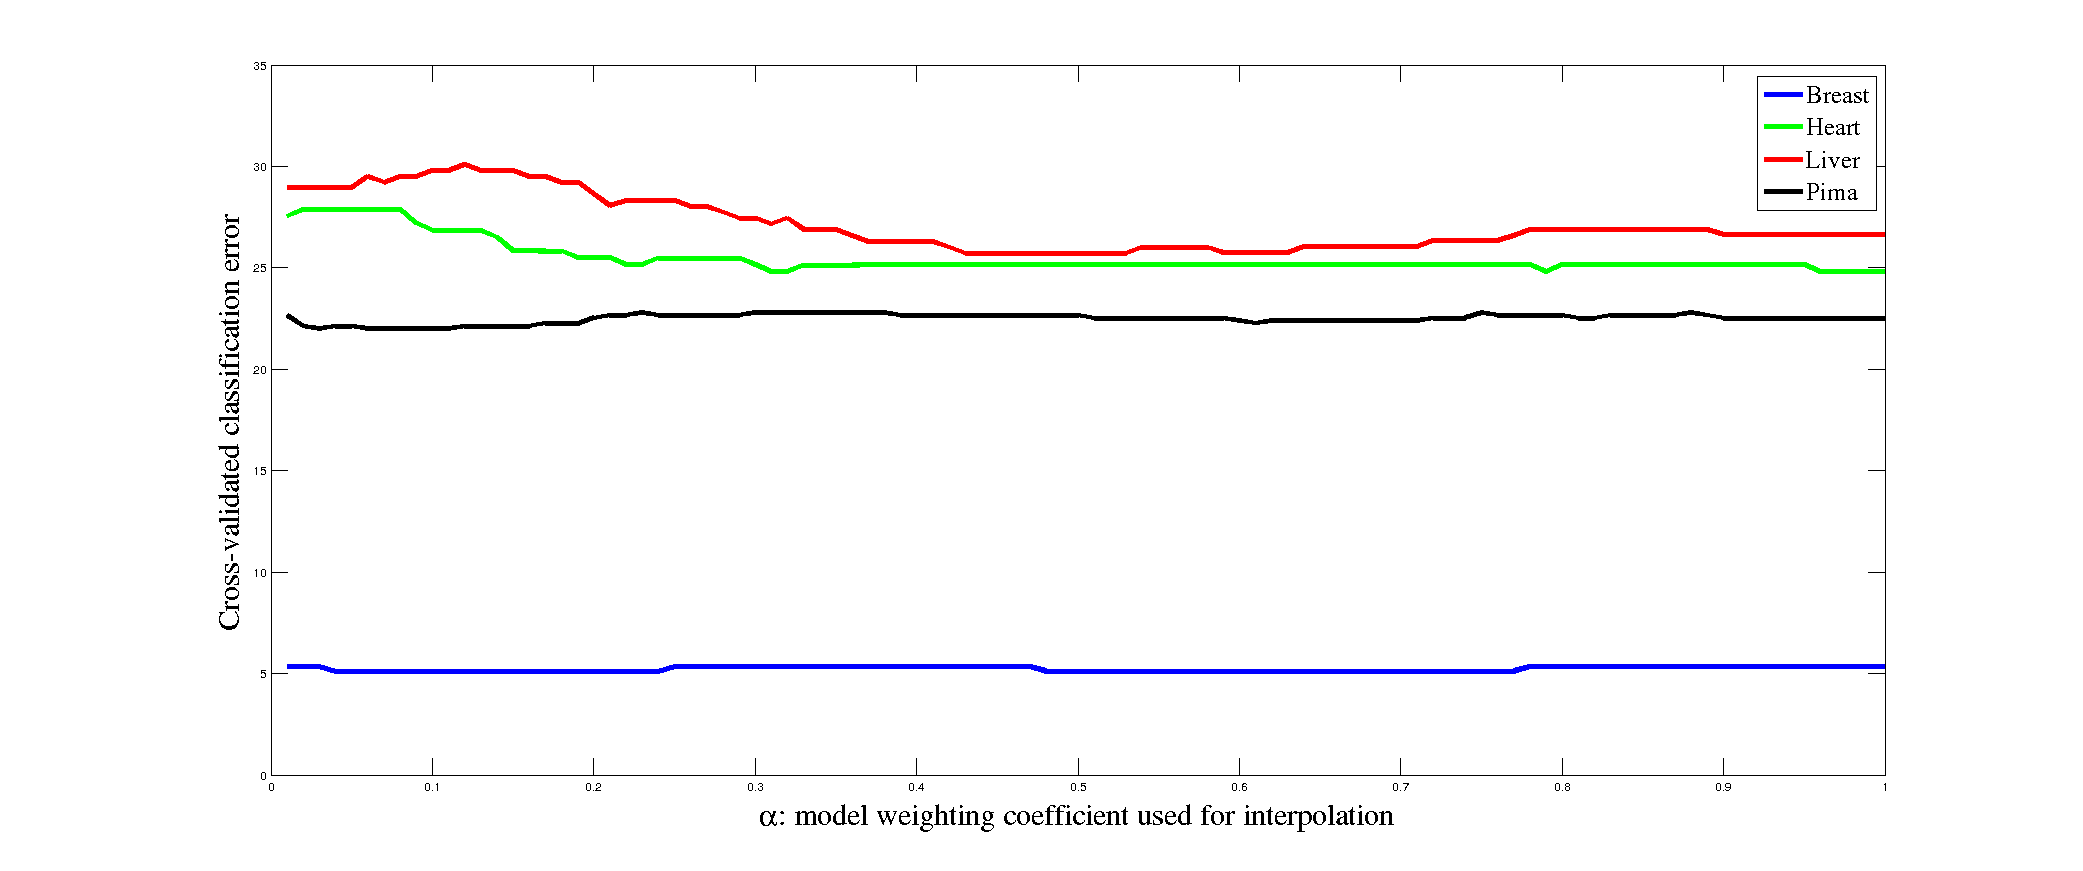
\includegraphics[trim=8cm 5cm 8cm 0cm, width=\textwidth]{figures/alphaBMA.png}%


\clearpage

\section{Providing Interpretability}

\subsection{Pima}

The Pima Indian Diabetes dataset contains medical measurements of 768 individuals, together with an indicator of whether they later developed diabetes or not. There are 8 attributes in total, 4 of which feature in the kernel structures returned by the kernel discovery procedure. 
These are dimensions 2, 6, 7 and 8: plasma glucose concentration, body mass index (BMI), diabetes pedigree function and the age of the patient. The remaining four attributes seem to carry less information regarding the likelihood of developing diabetes, at least 
in a dataset of this size and using this search procedure. These four features are the number of pregnancies, diastolic blood pressure, triceps skin fold thickness and 2-hour serum insulin measures. The structure returned most often (4 times using 10-fold cross validation 
for computing classification accuracy) was $[2\times7] + [6] + [8]$, closely followed by $[2]+[8]+[6 \times 7]$, which occured for 3 folds. The four posterior plots indicating the class boundaries determined with respect to these dimensions are shown below. 

\begin{center}

\makebox[(\textwidth) ]{
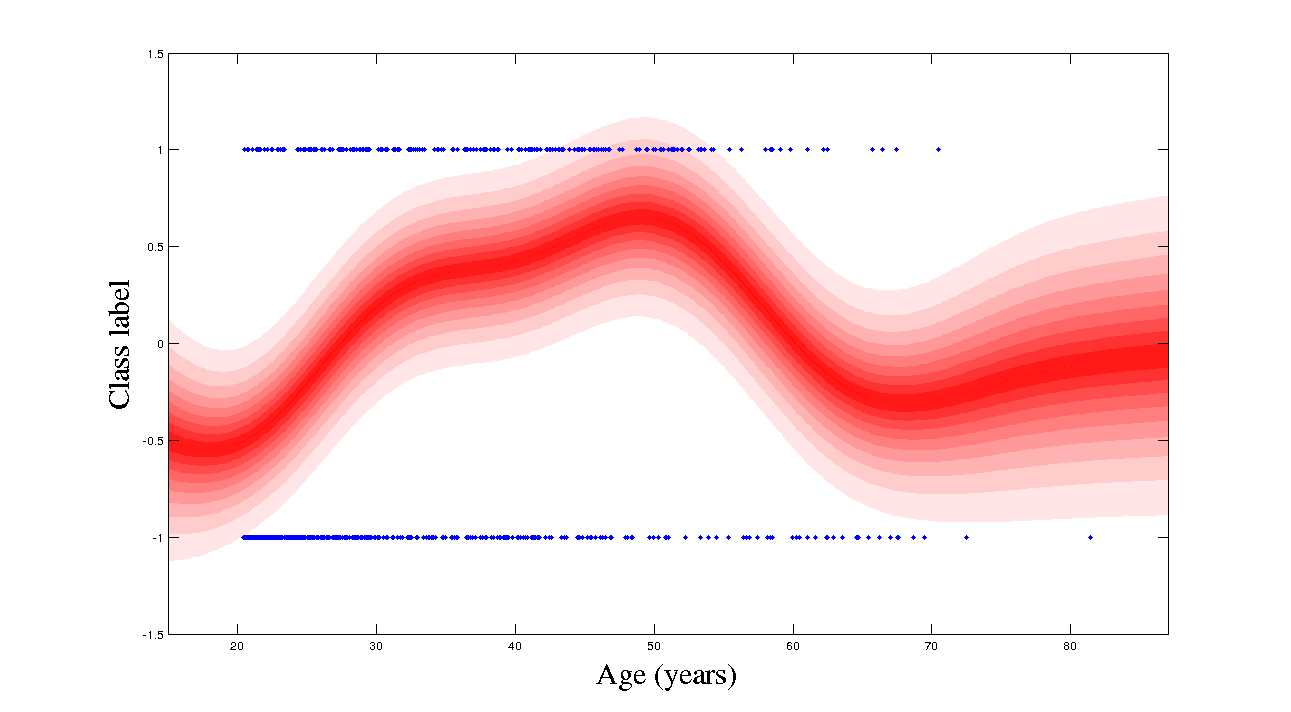
\includegraphics[trim=2cm 0cm 1cm 1cm, width=0.7\textwidth]{figures/pima/age.png}%
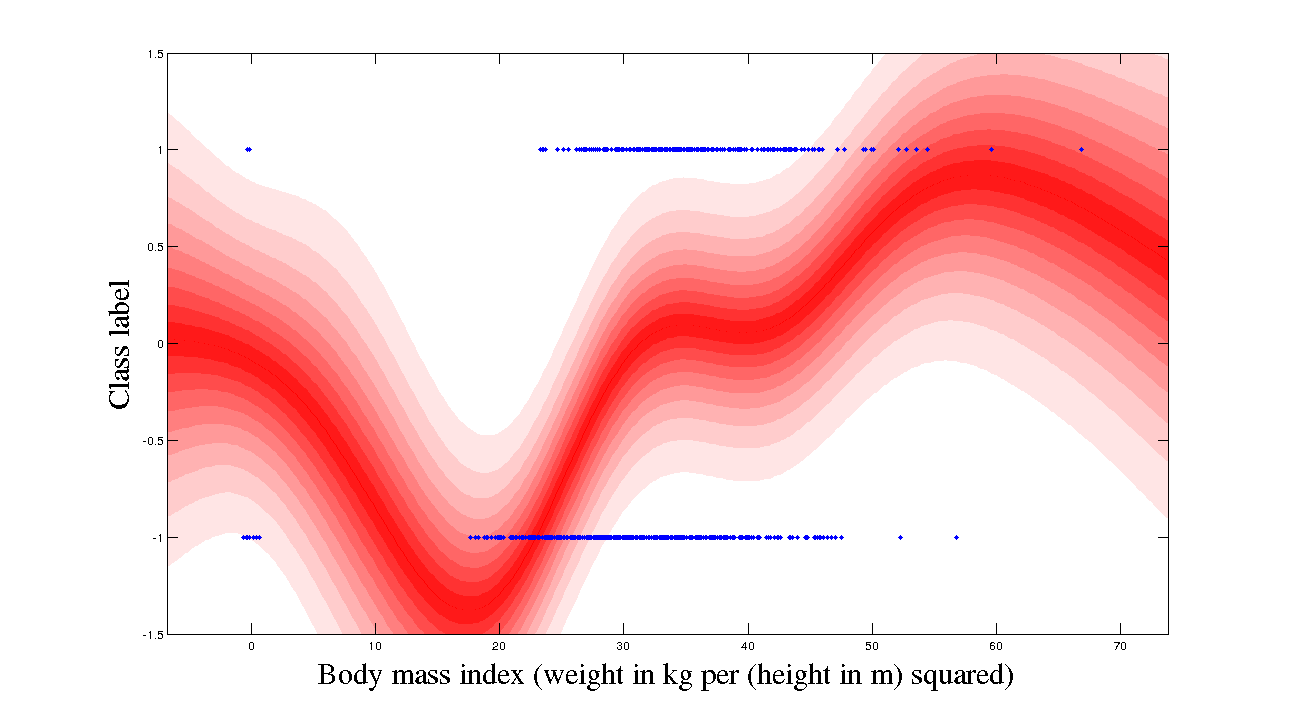
\includegraphics[trim=2cm 0cm 1cm 1cm, width=0.7\textwidth]{figures/pima/bmi.png}
}
\end{center}
\begin{center}
\makebox[(\textwidth) ]{
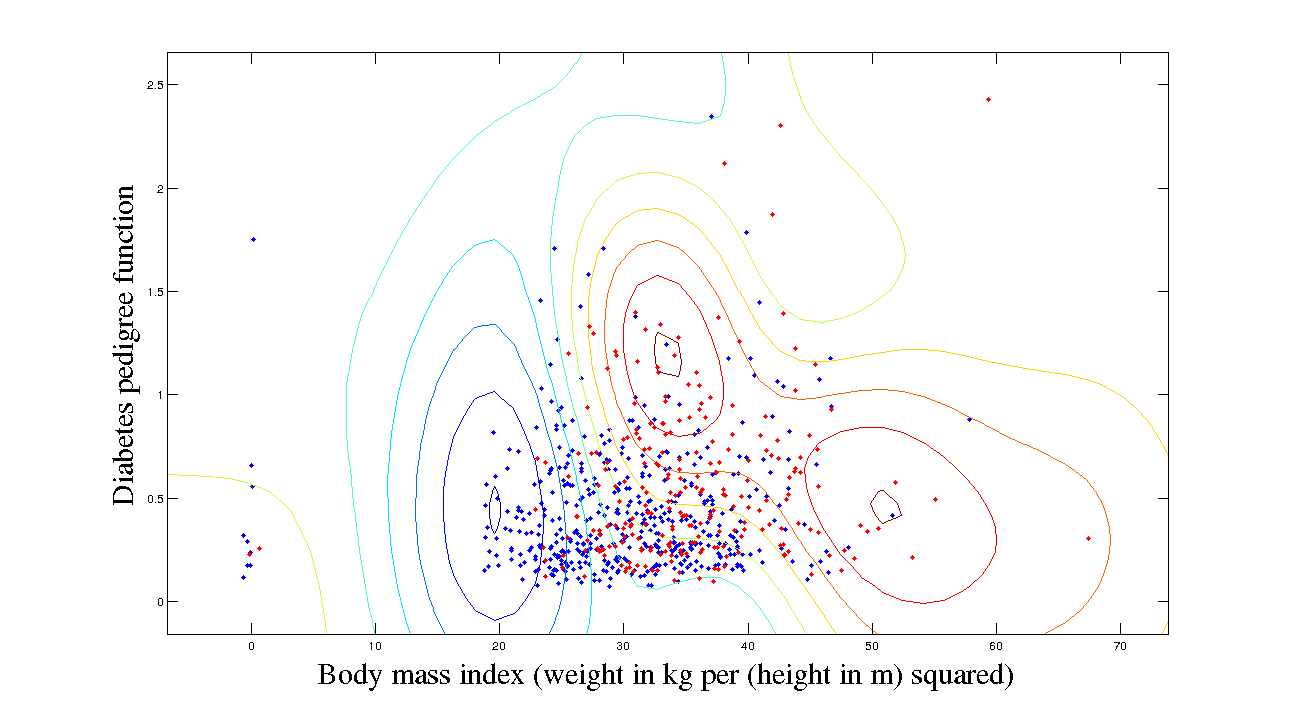
\includegraphics[trim=2cm 1cm 1cm 1cm, width=0.7\textwidth]{figures/pima/pedigreebmi.png}%
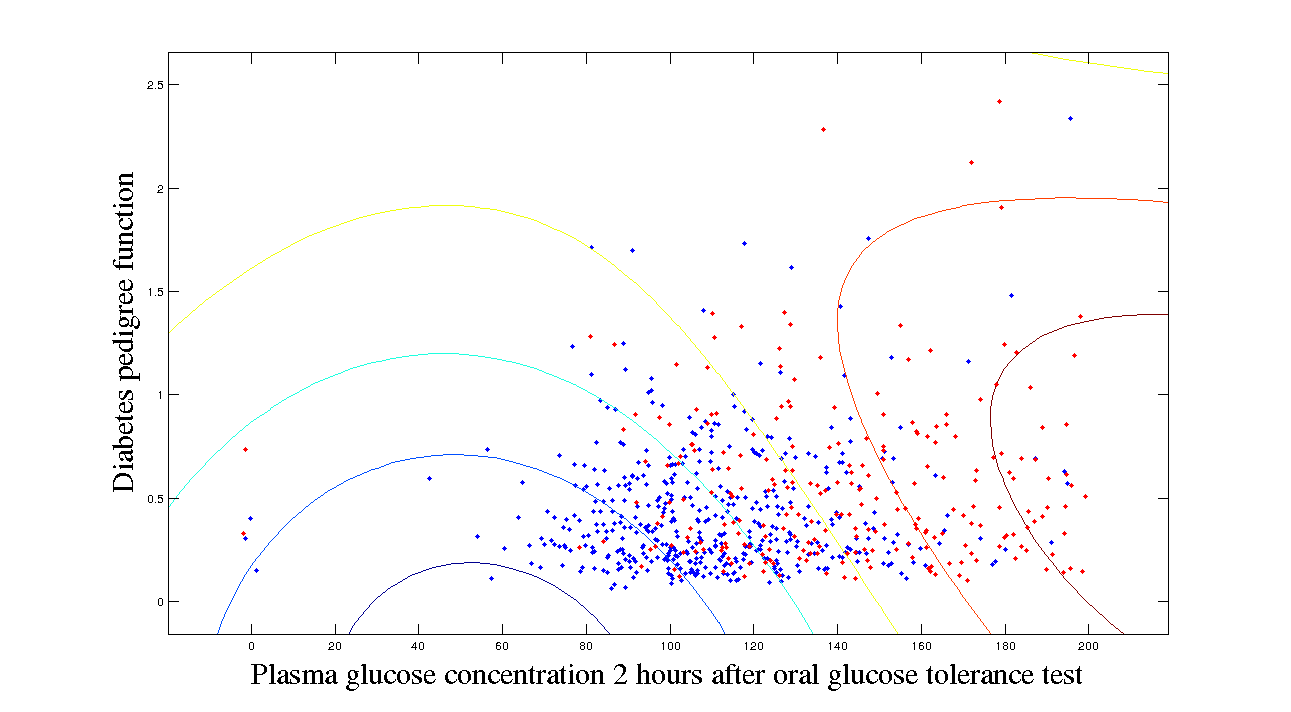
\includegraphics[trim=2cm 1cm 1cm 1cm, width=0.7\textwidth]{figures/pima/pedigreeglucose.png}
}
\end{center}

In addition to these additive components, the remaining three folds' structures contained occurances of $[2]$, $[2 \times 3 \times 7]$ and $ [ 2\times 3 \times7]$. Showing the three-way dependencies in 2D is not straightforward. Below, we show the posterior plots for 
$[2]$, $[2\times8]$ and $[3\times8]$, showing that interactions of these dimensions produce points well separated by the classifiers produced (with the possible exception of the interaction between age and diastolic blood pressure). The two way interaction between the number of pregnancies and age is also shown: this dependency was found during various 
stages of the search but discarded, even though the classifier seems to observe the general pattern present in the data set. 

\begin{center}
\makebox[(\textwidth) ]{
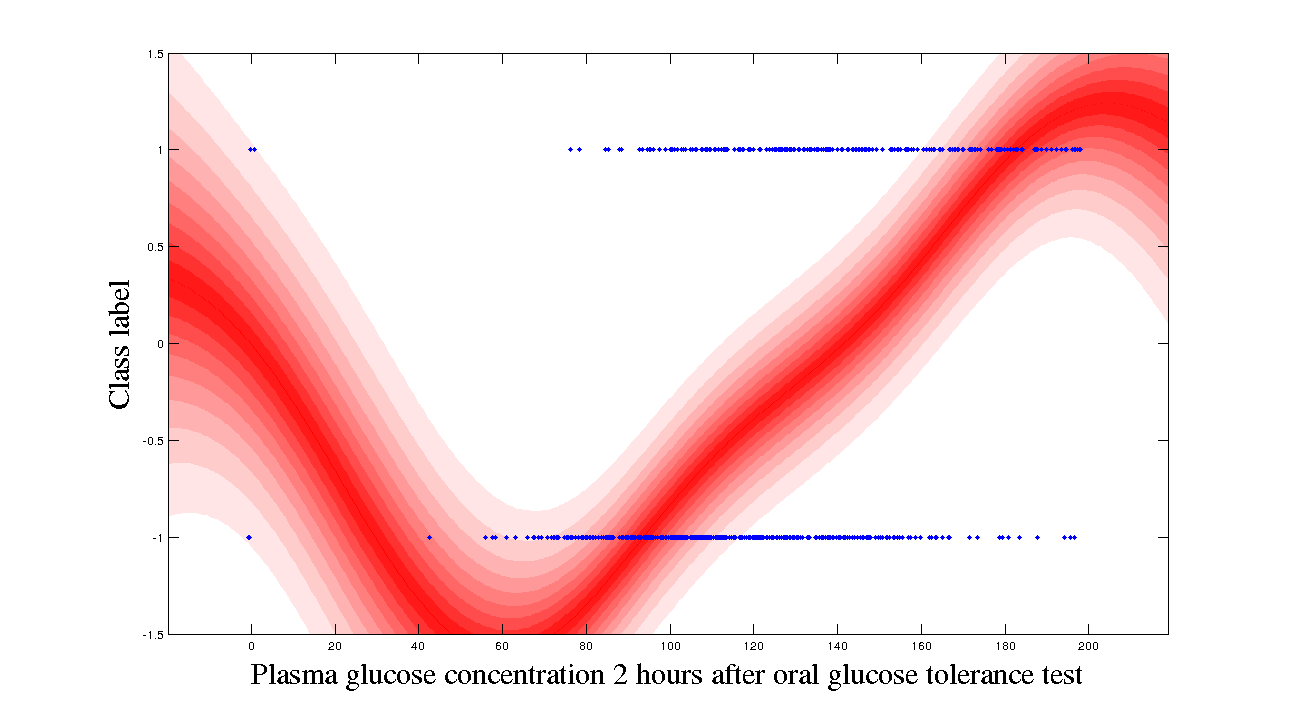
\includegraphics[trim=2cm 0cm 1cm 1cm, width=0.7\textwidth]{figures/pima/glucose.png}%
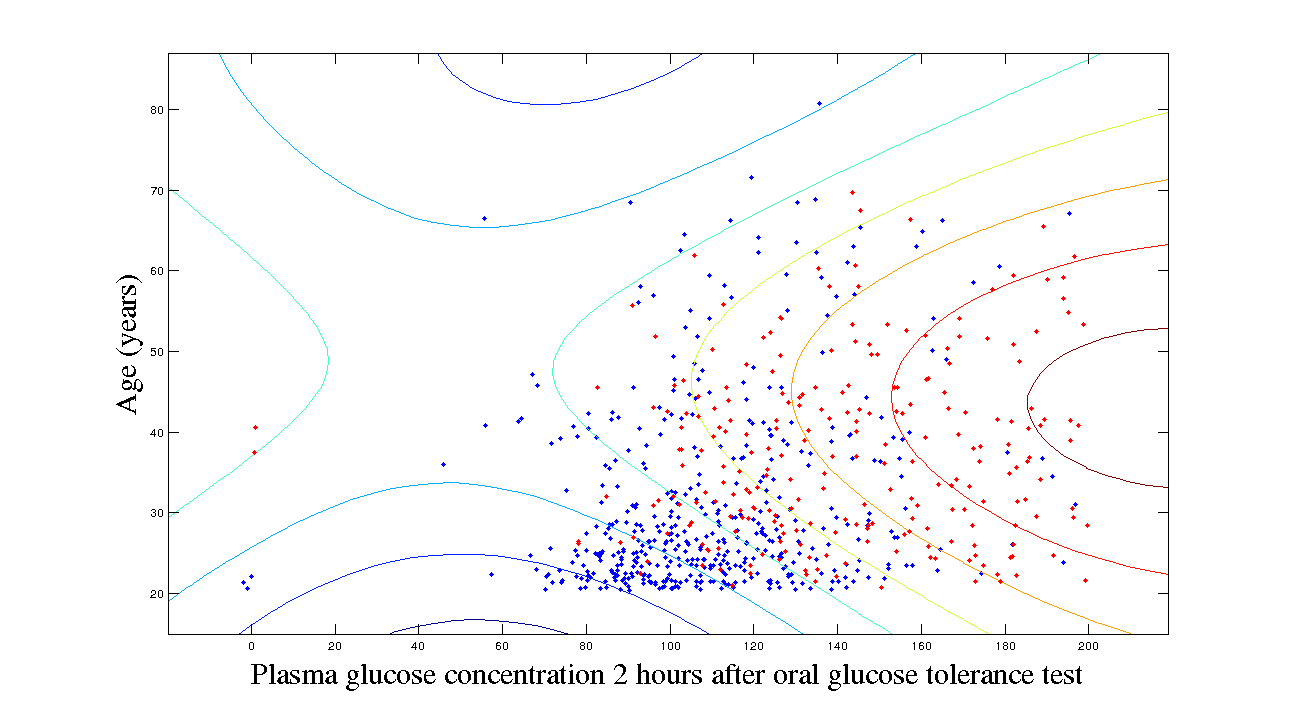
\includegraphics[trim=2cm 0cm 1cm 1cm, width=0.7\textwidth]{figures/pima/ageglucose.png}
}
\end{center}
\begin{center}

\makebox[(\textwidth) ]{
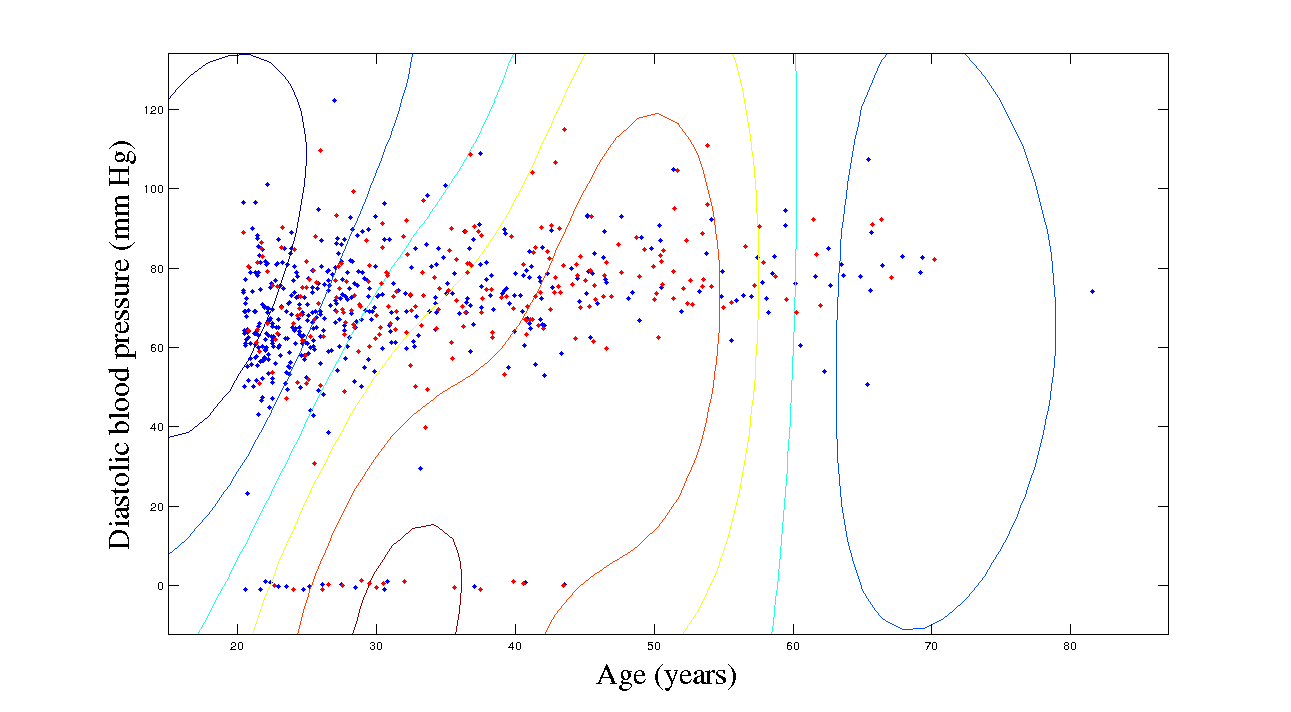
\includegraphics[trim=2cm 1cm 1cm 1cm, width=0.7\textwidth]{figures/pima/pressureage.png}
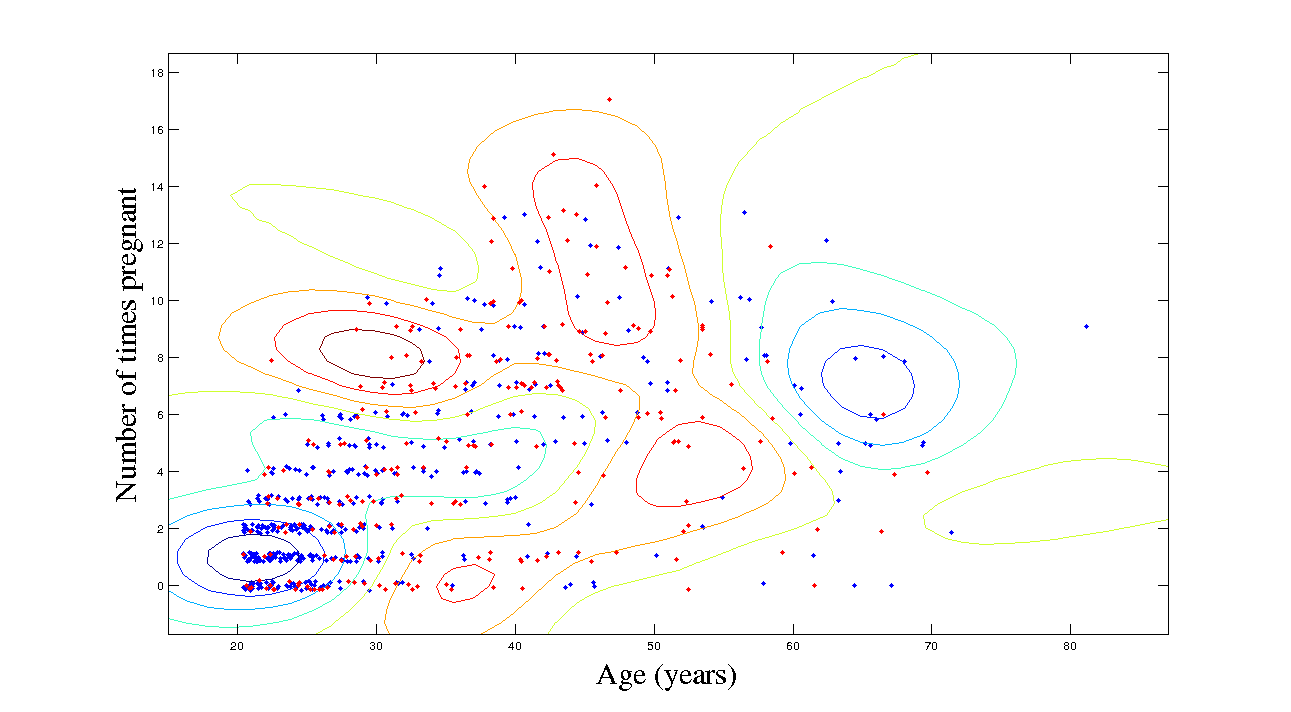
\includegraphics[trim=2cm 1cm 1cm 1cm, width=0.7\textwidth]{figures/pima/pregnantage.png}%
}
\end{center}

\subsection{Breast} 

Wisconsin Diagnostic Breast Cancer Dataset is a 9-dimensional dataset which contains measured attributes of 449 individuals, together with an indicator of whether or not they later developed breast cancer. Across the 10 folds generated, there were nine different kernel structures
that the procedure returned, with seven out of the nine attributes utilised in these structures. The dimensions most frequently found were 1, 2, 4, 6 and 8. Most kernels returned represent some combination of these five base kernels. Dimension 5 features once, and dimension 7 
three times. Interestingly, whenever $\SE_7$ was introduced, the accuracy increased far above the levels attained in the other kernels (ranging from 97\% to 100\%), but it was part of the final kernel in only three out of the ten folds evaluated. 

Below, we show those components of the 10 final structures which represent 1 or 2-way interactions. $[1 \times 2 \times 6]$ features in three folds, as do some other high dimensional interactions, but we are still unable to visualise those. 

The first six plots show individual components of the final kernel structures obtained using the structure search (not necessarily across the same fold). The final row shows dimensions 1 and 5 using a single $\SE$ kernel in the respective dimension. 


\begin{center}

\makebox[(\textwidth) ]{
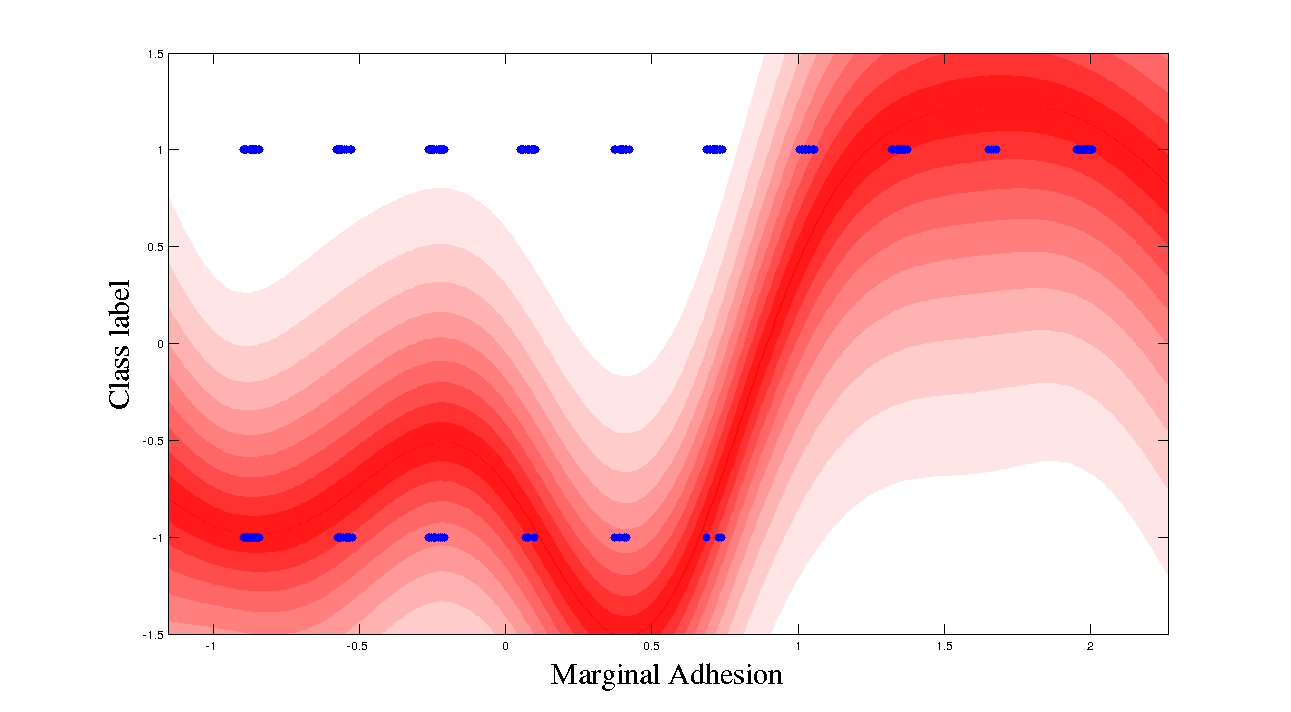
\includegraphics[trim=2cm 0cm 1cm 1cm, width=0.7\textwidth]{figures/breast/adhesion.png}%
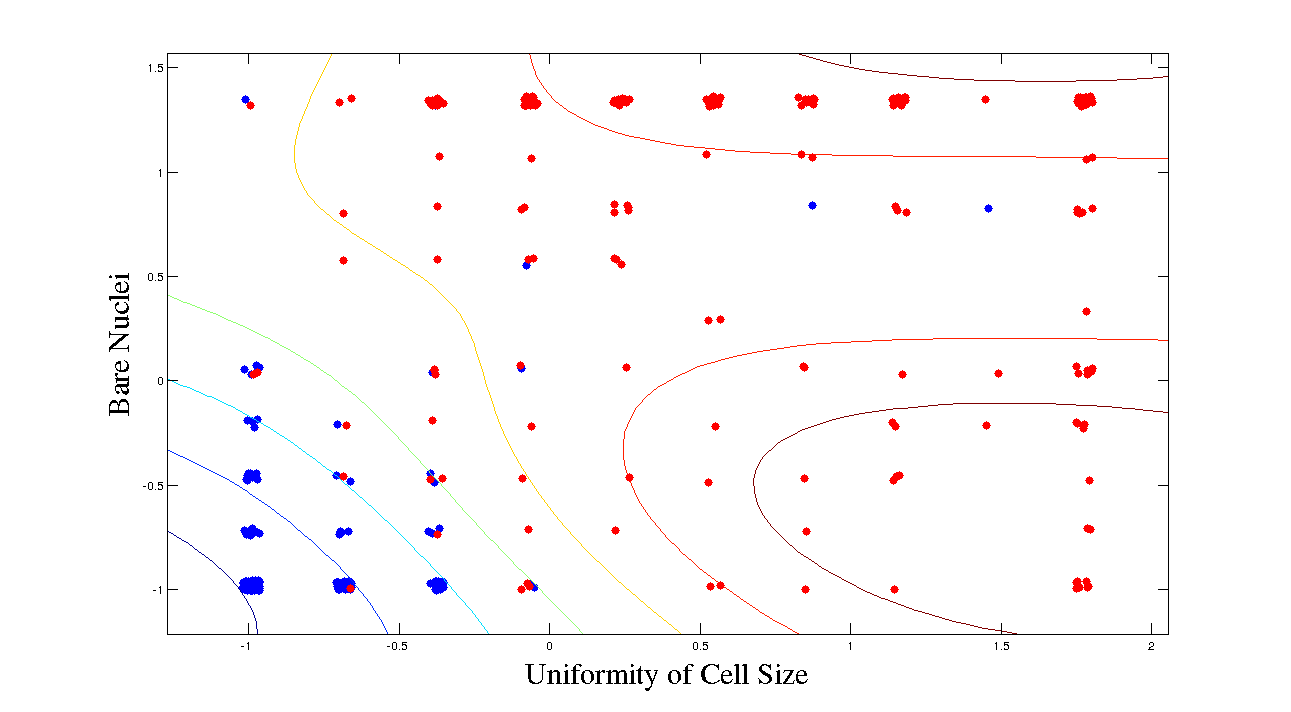
\includegraphics[trim=2cm 0cm 1cm 1cm, width=0.7\textwidth]{figures/breast/nucleicellsize.png}
}
\end{center}



\begin{center}
\makebox[(\textwidth) ]{
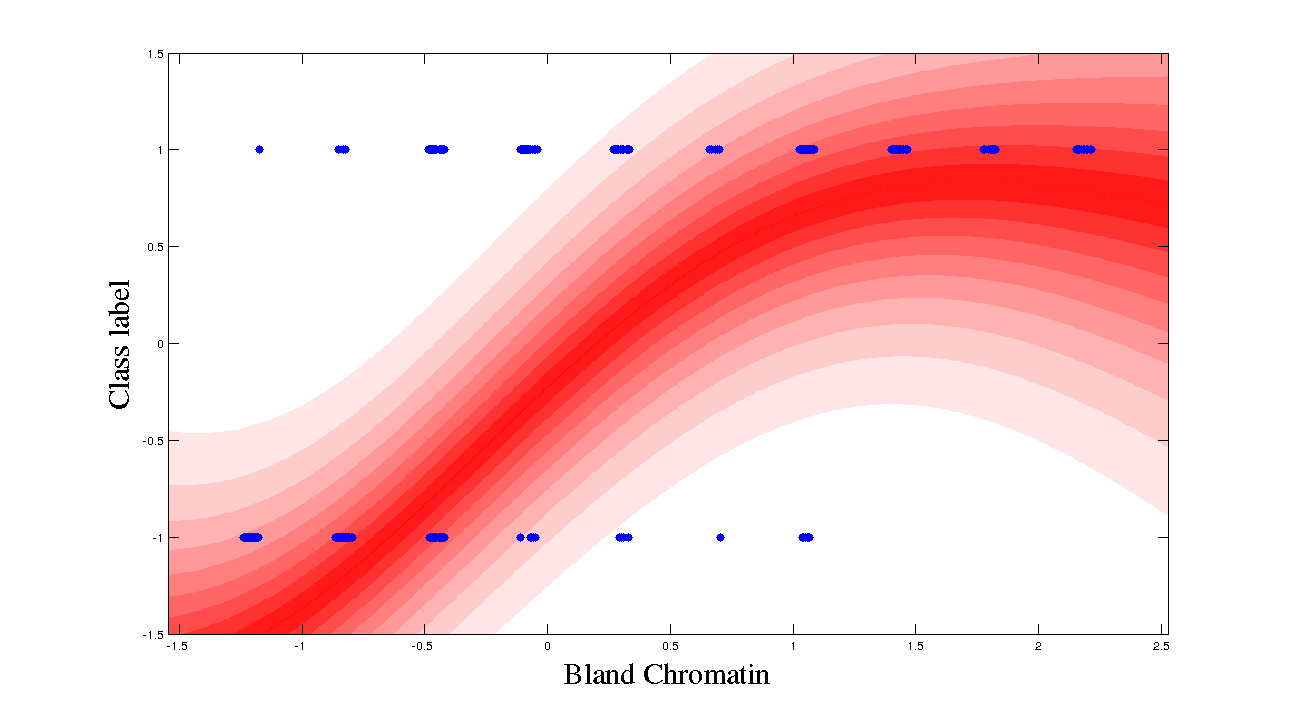
\includegraphics[trim=2cm 0cm 1cm 1cm, width=0.7\textwidth]{figures/breast/chromatin.png}%
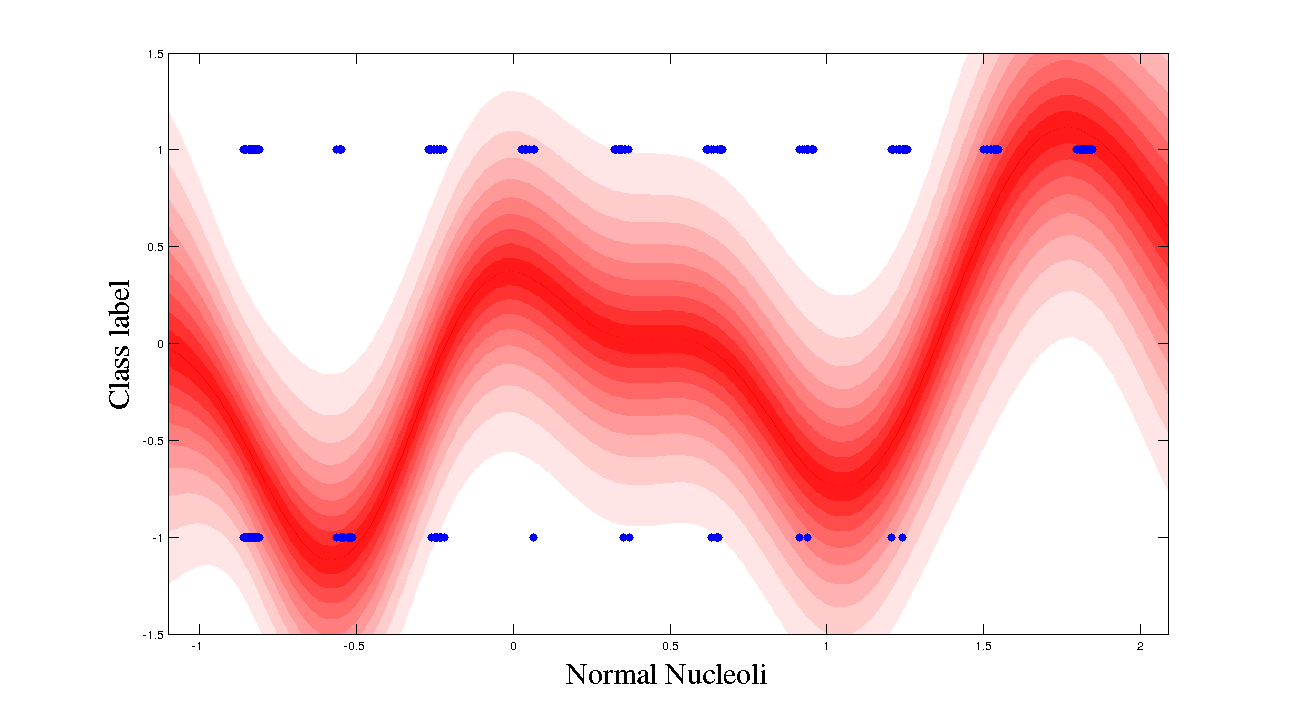
\includegraphics[trim=2cm 0cm 1cm 1cm, width=0.7\textwidth]{figures/breast/nucleoli.png}
}
\end{center}
\begin{center}


\makebox[(\textwidth) ]{
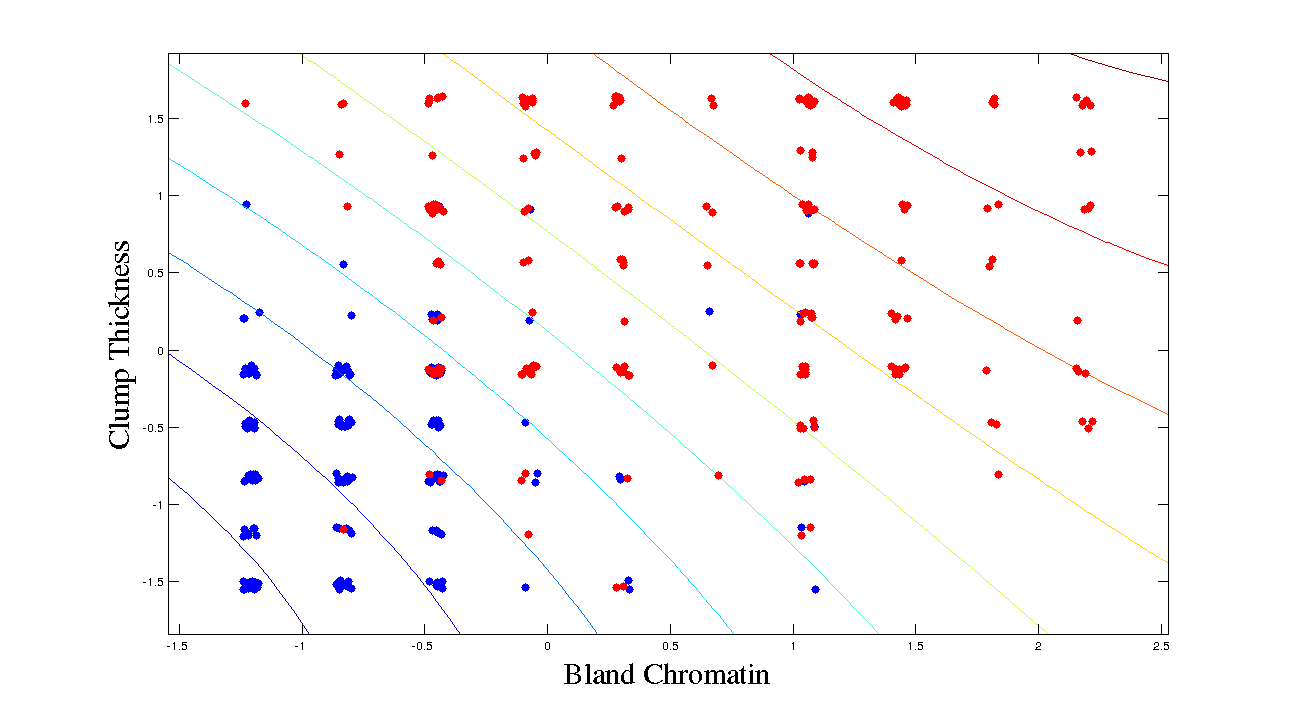
\includegraphics[trim=2cm 0cm 1cm 1cm, width=0.7\textwidth]{figures/breast/clumpbland.png}%
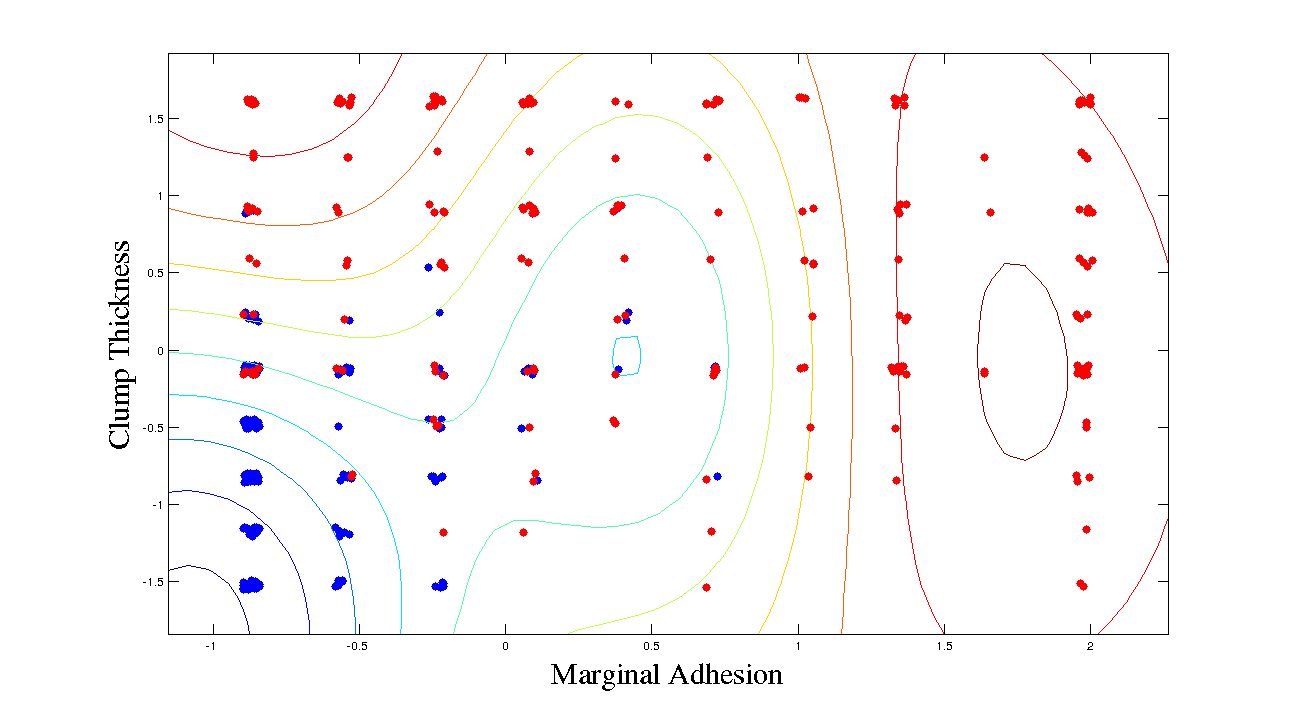
\includegraphics[trim=2cm 0cm 1cm 1cm, width=0.7\textwidth]{figures/breast/clumpadhesion.png}
}
\end{center}
\begin{center}

\makebox[(\textwidth) ]{
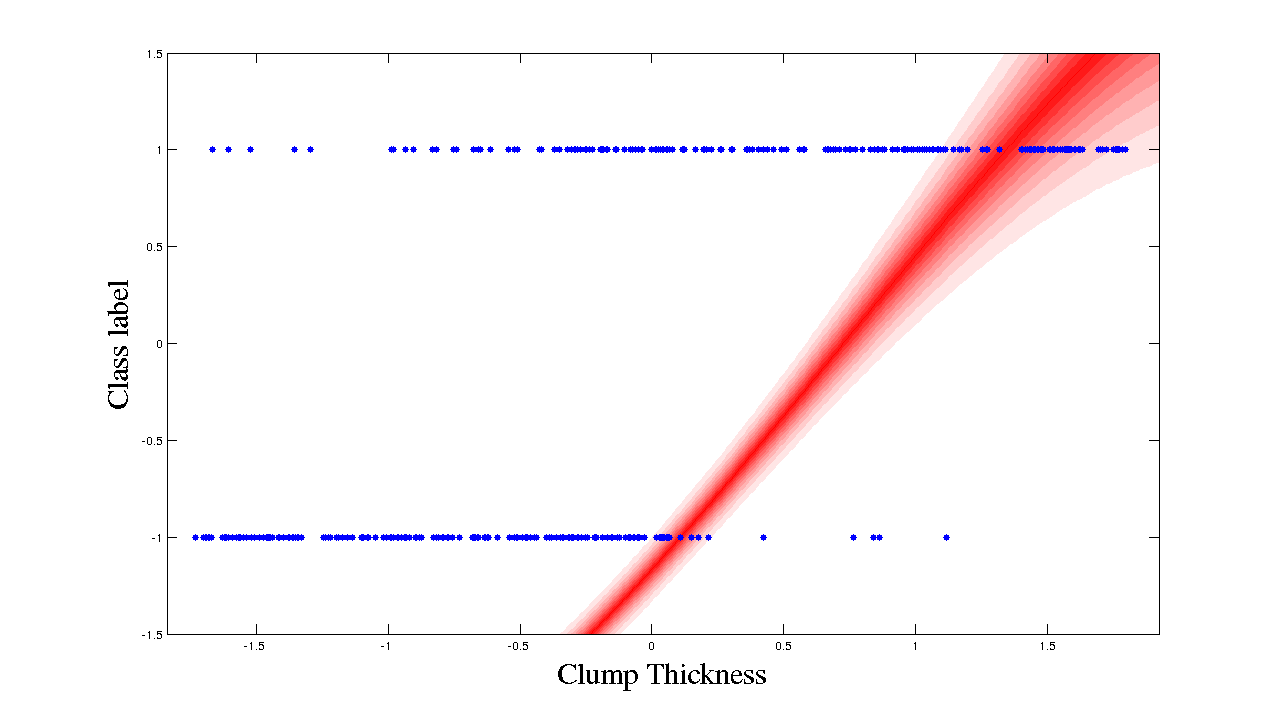
\includegraphics[trim=2cm 0cm 1cm 1cm, width=0.7\textwidth]{figures/breast/clump.png}%
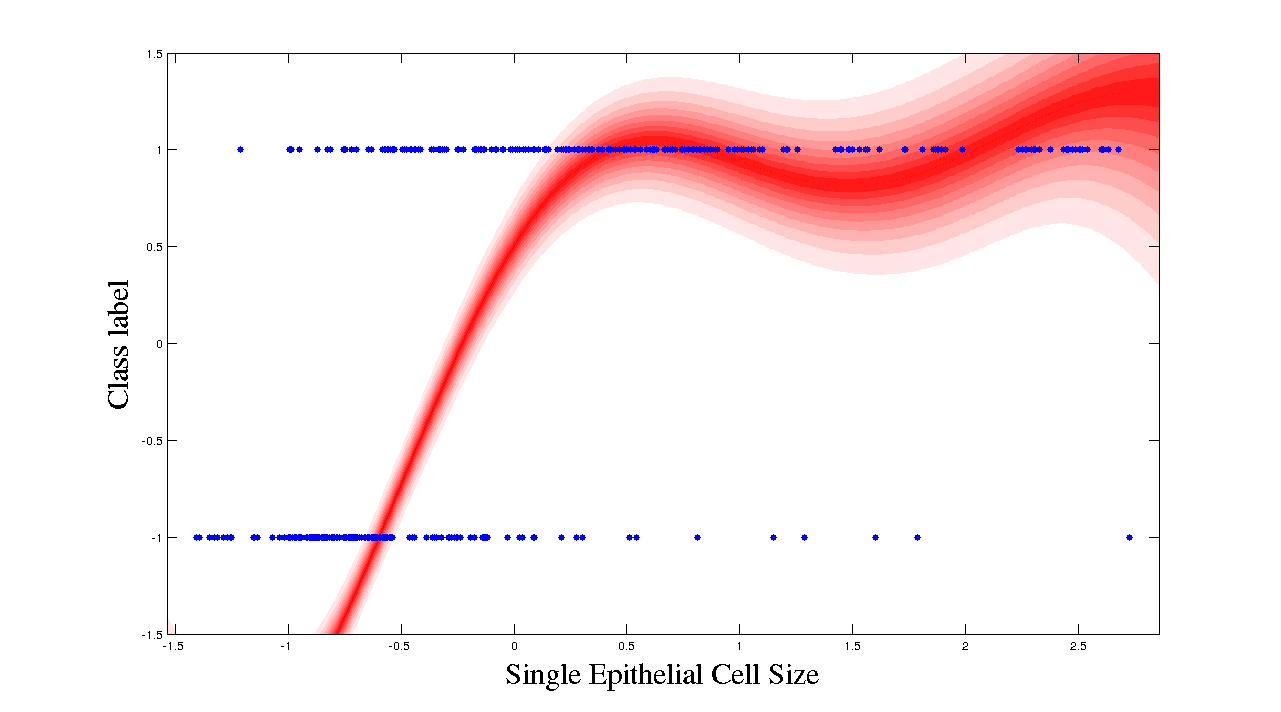
\includegraphics[trim=2cm 0cm 1cm 1cm, width=0.7\textwidth]{figures/breast/cellsize.png}
}
\end{center}


% \subsection{Heart and Liver}
% These two data sets require dealing with representation of discretised data. Plots don't make much sense (yet). Adding jitter might alleviate these issues.  


% \clearpage

% \section{Automatic Report Generation}



\begin{comment}

\subsection{BMA/Cross-validated model for Model Selection}

Choosing the most frequently occuring model structure, then optimising hyperparametees on each training fold and evaluating on the respective test fold gets the following figures:

\subsection{Liver}

Kernel chosen for this data set is: $ \SE_1 + \SE_3 \times \SE_4 \times \SE_5 + \SE_6 $, and the testing errors on the ten folds are: 

\begin{table}[h]

  \begin{tabular}{|c | c  | }
      \hline
      \multicolumn{2}{|c|}{Liver}  \\
      \hline
      Per-fold models & `Best' model \\  \hline
23.53\%	& 23.53\% \\ 
20.00\%	& 20.00\% \\
37.14\%	& 37.14\% \\
40.00\%	& \textbf{34.29\%} \\
28.57\%	& 34.29\% \\
26.47\%	& \textbf{23.53\%} \\
23.53\%	& 26.47\% \\
26.47\%	& 26.47\% \\
25.71\%	& 25.71\% \\
23.53\%	& \textbf{14.71\%} \\ \hline \hline
27.50\%	& \textbf{26.61\%} \\

      \hline 
      \end{tabular}
\end{table}

   The average error is $26.61 \%$, which improves on the previous value of $27.5\%$, but falls short of using weighted model averaging. 

For breast, picking $ [ 1 \times 2 \times 6 + 7 ] $ leads to the following performance, yielding an improvement of $0.9\%$ over the standard BIC light version. 

\begin{table}[h]

  \begin{tabular}{|c | }
      \hline
      \multicolumn{1}{|c|}{Breast}  \\
      \hline
       `Best' model \\  \hline
2.27\% \\
4.55\%\\
11.11\%\\
11.11\%\\
2.27\%\\
10.87\%\\
0.00\%\\
2.22\%\\
4.35\%\\
6.67\%\\

      \hline 
      \end{tabular}
\end{table}

\end{comment}


\chapter{Summary and Conclusions} 

%As you might imagine: summarizes the dissertation, and draws any conclusions. Depending on the length of your work, and how well you write, you may not need a summary here. 
%You will generally want to draw some conclusions, and point to potential future work. 

\section{Further Work}

\clearpage


\appendix
\singlespacing

\bibliographystyle{unsrt} 
\bibliography{refs} 

\end{document}